\documentclass[1p]{elsarticle_modified}
%\bibliographystyle{elsarticle-num}

%\usepackage[colorlinks]{hyperref}
%\usepackage{abbrmath_seonhwa} %\Abb, \Ascr, \Acal ,\Abf, \Afrak
\usepackage{amsfonts}
\usepackage{amssymb}
\usepackage{amsmath}
\usepackage{amsthm}
\usepackage{scalefnt}
\usepackage{amsbsy}
\usepackage{kotex}
\usepackage{caption}
\usepackage{subfig}
\usepackage{color}
\usepackage{graphicx}
\usepackage{xcolor} %% white, black, red, green, blue, cyan, magenta, yellow
\usepackage{float}
\usepackage{setspace}
\usepackage{hyperref}

\usepackage{tikz}
\usetikzlibrary{arrows}

\usepackage{multirow}
\usepackage{array} % fixed length table
\usepackage{hhline}

%%%%%%%%%%%%%%%%%%%%%
\makeatletter
\renewcommand*\env@matrix[1][\arraystretch]{%
	\edef\arraystretch{#1}%
	\hskip -\arraycolsep
	\let\@ifnextchar\new@ifnextchar
	\array{*\c@MaxMatrixCols c}}
\makeatother %https://tex.stackexchange.com/questions/14071/how-can-i-increase-the-line-spacing-in-a-matrix
%%%%%%%%%%%%%%%

\usepackage[normalem]{ulem}

\newcommand{\msout}[1]{\ifmmode\text{\sout{\ensuremath{#1}}}\else\sout{#1}\fi}
%SOURCE: \msout is \stkout macro in https://tex.stackexchange.com/questions/20609/strikeout-in-math-mode

\newcommand{\cancel}[1]{
	\ifmmode
	{\color{red}\msout{#1}}
	\else
	{\color{red}\sout{#1}}
	\fi
}

\newcommand{\add}[1]{
	{\color{blue}\uwave{#1}}
}

\newcommand{\replace}[2]{
	\ifmmode
	{\color{red}\msout{#1}}{\color{blue}\uwave{#2}}
	\else
	{\color{red}\sout{#1}}{\color{blue}\uwave{#2}}
	\fi
}

\newcommand{\Sol}{\mathcal{S}} %segment
\newcommand{\D}{D} %diagram
\newcommand{\A}{\mathcal{A}} %arc


%%%%%%%%%%%%%%%%%%%%%%%%%%%%%5 test

\def\sl{\operatorname{\textup{SL}}(2,\Cbb)}
\def\psl{\operatorname{\textup{PSL}}(2,\Cbb)}
\def\quan{\mkern 1mu \triangleright \mkern 1mu}

\theoremstyle{definition}
\newtheorem{thm}{Theorem}[section]
\newtheorem{prop}[thm]{Proposition}
\newtheorem{lem}[thm]{Lemma}
\newtheorem{ques}[thm]{Question}
\newtheorem{cor}[thm]{Corollary}
\newtheorem{defn}[thm]{Definition}
\newtheorem{exam}[thm]{Example}
\newtheorem{rmk}[thm]{Remark}
\newtheorem{alg}[thm]{Algorithm}

\newcommand{\I}{\sqrt{-1}}
\begin{document}

%\begin{frontmatter}
%
%\title{Boundary parabolic representations of knots up to 8 crossings}
%
%%% Group authors per affiliation:
%\author{Yunhi Cho} 
%\address{Department of Mathematics, University of Seoul, Seoul, Korea}
%\ead{yhcho@uos.ac.kr}
%
%
%\author{Seonhwa Kim} %\fnref{s_kim}}
%\address{Center for Geometry and Physics, Institute for Basic Science, Pohang, 37673, Korea}
%\ead{ryeona17@ibs.re.kr}
%
%\author{Hyuk Kim}
%\address{Department of Mathematical Sciences, Seoul National University, Seoul 08826, Korea}
%\ead{hyukkim@snu.ac.kr}
%
%\author{Seokbeom Yoon}
%\address{Department of Mathematical Sciences, Seoul National University, Seoul, 08826,  Korea}
%\ead{sbyoon15@snu.ac.kr}
%
%\begin{abstract}
%We find all boundary parabolic representation of knots up to 8 crossings.
%
%\end{abstract}
%\begin{keyword}
%    \MSC[2010] 57M25 
%\end{keyword}
%
%\end{frontmatter}

%\linenumbers
%\tableofcontents
%
\newcommand\colored[1]{\textcolor{white}{\rule[-0.35ex]{0.8em}{1.4ex}}\kern-0.8em\color{red} #1}%
%\newcommand\colored[1]{\textcolor{white}{ #1}\kern-2.17ex	\textcolor{white}{ #1}\kern-1.81ex	\textcolor{white}{ #1}\kern-2.15ex\color{red}#1	}

{\Large $\underline{12a_{1270}~(K12a_{1270})}$}

\setlength{\tabcolsep}{10pt}
\renewcommand{\arraystretch}{1.6}
\vspace{1cm}\begin{tabular}{m{100pt}>{\centering\arraybackslash}m{274pt}}
\multirow{5}{120pt}{
	\centering
	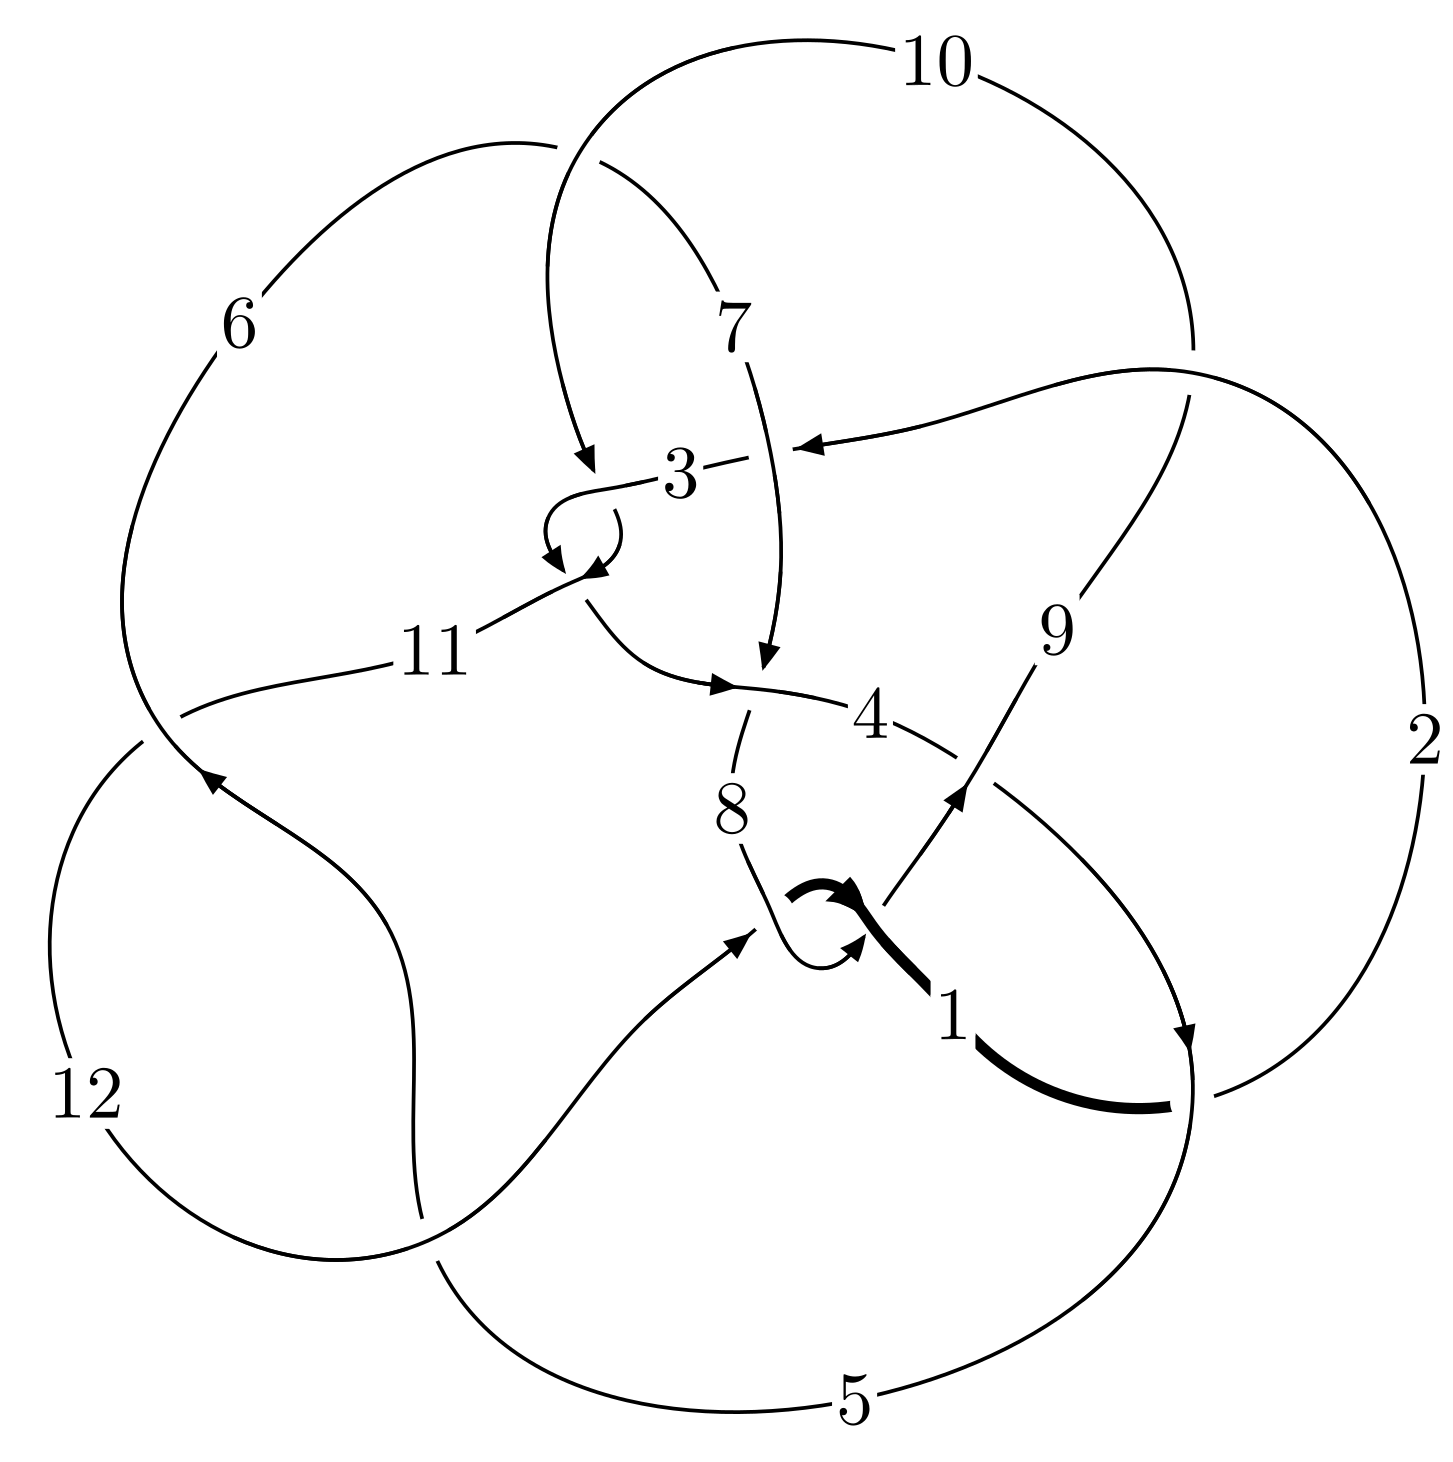
\includegraphics[width=112pt]{../../../GIT/diagram.site/Diagrams/png/2071_12a_1270.png}\\
\ \ \ A knot diagram\footnotemark}&
\allowdisplaybreaks
\textbf{Linearized knot diagam} \\
\cline{2-2}
 &
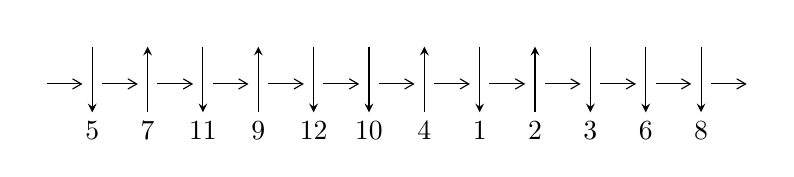
\begin{tikzpicture}[x=20pt, y=17pt]
	% nodes
	\node (C0) at (0, 0) {};
	\node (C1) at (1, 0) {};
	\node (C1U) at (1, +1) {};
	\node (C1D) at (1, -1) {5};

	\node (C2) at (2, 0) {};
	\node (C2U) at (2, +1) {};
	\node (C2D) at (2, -1) {7};

	\node (C3) at (3, 0) {};
	\node (C3U) at (3, +1) {};
	\node (C3D) at (3, -1) {11};

	\node (C4) at (4, 0) {};
	\node (C4U) at (4, +1) {};
	\node (C4D) at (4, -1) {9};

	\node (C5) at (5, 0) {};
	\node (C5U) at (5, +1) {};
	\node (C5D) at (5, -1) {12};

	\node (C6) at (6, 0) {};
	\node (C6U) at (6, +1) {};
	\node (C6D) at (6, -1) {10};

	\node (C7) at (7, 0) {};
	\node (C7U) at (7, +1) {};
	\node (C7D) at (7, -1) {4};

	\node (C8) at (8, 0) {};
	\node (C8U) at (8, +1) {};
	\node (C8D) at (8, -1) {1};

	\node (C9) at (9, 0) {};
	\node (C9U) at (9, +1) {};
	\node (C9D) at (9, -1) {2};

	\node (C10) at (10, 0) {};
	\node (C10U) at (10, +1) {};
	\node (C10D) at (10, -1) {3};

	\node (C11) at (11, 0) {};
	\node (C11U) at (11, +1) {};
	\node (C11D) at (11, -1) {6};

	\node (C12) at (12, 0) {};
	\node (C12U) at (12, +1) {};
	\node (C12D) at (12, -1) {8};
	\node (C13) at (13, 0) {};

	% arrows
	\draw[->,>={angle 60}]
	(C0) edge (C1) (C1) edge (C2) (C2) edge (C3) (C3) edge (C4) (C4) edge (C5) (C5) edge (C6) (C6) edge (C7) (C7) edge (C8) (C8) edge (C9) (C9) edge (C10) (C10) edge (C11) (C11) edge (C12) (C12) edge (C13) ;	\draw[->,>=stealth]
	(C1U) edge (C1D) (C2D) edge (C2U) (C3U) edge (C3D) (C4D) edge (C4U) (C5U) edge (C5D) (C6U) edge (C6D) (C7D) edge (C7U) (C8U) edge (C8D) (C9D) edge (C9U) (C10U) edge (C10D) (C11U) edge (C11D) (C12U) edge (C12D) ;
	\end{tikzpicture} \\
\hhline{~~} \\& 
\textbf{Solving Sequence} \\ \cline{2-2} 
 &
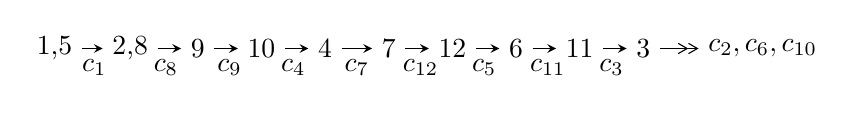
\begin{tikzpicture}[x=23pt, y=7pt]
	% node
	\node (A0) at (-1/8, 0) {1,5};
	\node (A1) at (17/16, 0) {2,8};
	\node (A2) at (17/8, 0) {9};
	\node (A3) at (25/8, 0) {10};
	\node (A4) at (33/8, 0) {4};
	\node (A5) at (41/8, 0) {7};
	\node (A6) at (49/8, 0) {12};
	\node (A7) at (57/8, 0) {6};
	\node (A8) at (65/8, 0) {11};
	\node (A9) at (73/8, 0) {3};
	\node (C1) at (1/2, -1) {$c_{1}$};
	\node (C2) at (13/8, -1) {$c_{8}$};
	\node (C3) at (21/8, -1) {$c_{9}$};
	\node (C4) at (29/8, -1) {$c_{4}$};
	\node (C5) at (37/8, -1) {$c_{7}$};
	\node (C6) at (45/8, -1) {$c_{12}$};
	\node (C7) at (53/8, -1) {$c_{5}$};
	\node (C8) at (61/8, -1) {$c_{11}$};
	\node (C9) at (69/8, -1) {$c_{3}$};
	\node (A10) at (11, 0) {$c_{2},c_{6},c_{10}$};

	% edge
	\draw[->,>=stealth]	
	(A0) edge (A1) (A1) edge (A2) (A2) edge (A3) (A3) edge (A4) (A4) edge (A5) (A5) edge (A6) (A6) edge (A7) (A7) edge (A8) (A8) edge (A9) ;
	\draw[->>,>={angle 60}]	
	(A9) edge (A10);
\end{tikzpicture} \\ 

\end{tabular} \\

\footnotetext{
The image of knot diagram is generated by the software ``\textbf{Draw programme}" developed by Andrew Bartholomew(\url{http://www.layer8.co.uk/maths/draw/index.htm\#Running-draw}), where we modified some parts for our purpose(\url{https://github.com/CATsTAILs/LinksPainter}).
}\phantom \\ \newline 
\centering \textbf{Ideals for irreducible components\footnotemark of $X_{\text{par}}$} 
 
\begin{align*}
I^u_{1}&=\langle 
7.74082\times10^{49} u^{34}-5.22423\times10^{49} u^{33}+\cdots+1.89535\times10^{51} b-5.14492\times10^{51},\\
\phantom{I^u_{1}}&\phantom{= \langle  }-9.06527\times10^{50} u^{34}+2.64032\times10^{50} u^{33}+\cdots+1.13721\times10^{52} a+6.01325\times10^{52},\\
\phantom{I^u_{1}}&\phantom{= \langle  }u^{35}- u^{34}+\cdots-72 u+24\rangle \\
I^u_{2}&=\langle 
2.37244\times10^{960} u^{121}-2.53157\times10^{961} u^{120}+\cdots+2.07793\times10^{963} b+5.97659\times10^{962},\\
\phantom{I^u_{2}}&\phantom{= \langle  }6.58503\times10^{963} u^{121}-6.71449\times10^{964} u^{120}+\cdots+2.59741\times10^{965} a-3.63631\times10^{966},\\
\phantom{I^u_{2}}&\phantom{= \langle  }u^{122}-10 u^{121}+\cdots-1165 u-125\rangle \\
I^u_{3}&=\langle 
-5.91071\times10^{45} u^{25}+3.90400\times10^{46} u^{24}+\cdots+1.44135\times10^{48} b-5.25354\times10^{46},\\
\phantom{I^u_{3}}&\phantom{= \langle  }-7.34230\times10^{46} u^{25}+5.10520\times10^{47} u^{24}+\cdots+2.59442\times10^{49} a-7.68850\times10^{48},\\
\phantom{I^u_{3}}&\phantom{= \langle  }u^{26}-5 u^{25}+\cdots+72 u+72\rangle \\
I^u_{4}&=\langle 
- u^4-2 u^3-2 u^2+b+u+2,\;u^4+u^3+2 u^2+a- u,\;u^5+u^4+u^3-2 u^2- u+1\rangle \\
\\
I^v_{1}&=\langle 
a,\;b-1,\;v-1\rangle \\
\end{align*}
\raggedright * 5 irreducible components of $\dim_{\mathbb{C}}=0$, with total 189 representations.\\
\footnotetext{All coefficients of polynomials are rational numbers. But the coefficients are sometimes approximated in decimal forms when there is not enough margin.}
\newpage
\renewcommand{\arraystretch}{1}
\centering \section*{I. $I^u_{1}= \langle 7.74\times10^{49} u^{34}-5.22\times10^{49} u^{33}+\cdots+1.90\times10^{51} b-5.14\times10^{51},\;-9.07\times10^{50} u^{34}+2.64\times10^{50} u^{33}+\cdots+1.14\times10^{52} a+6.01\times10^{52},\;u^{35}- u^{34}+\cdots-72 u+24 \rangle$}
\flushleft \textbf{(i) Arc colorings}\\
\begin{tabular}{m{7pt} m{180pt} m{7pt} m{180pt} }
\flushright $a_{1}=$&$\begin{pmatrix}1\\0\end{pmatrix}$ \\
\flushright $a_{5}=$&$\begin{pmatrix}0\\u\end{pmatrix}$ \\
\flushright $a_{2}=$&$\begin{pmatrix}1\\u^2\end{pmatrix}$ \\
\flushright $a_{8}=$&$\begin{pmatrix}0.0797150 u^{34}-0.0232175 u^{33}+\cdots+6.72639 u-5.28772\\-0.0408411 u^{34}+0.0275634 u^{33}+\cdots+1.10469 u+2.71450\end{pmatrix}$ \\
\flushright $a_{9}=$&$\begin{pmatrix}0.120556 u^{34}-0.0507809 u^{33}+\cdots+5.62170 u-8.00222\\-0.0408411 u^{34}+0.0275634 u^{33}+\cdots+1.10469 u+2.71450\end{pmatrix}$ \\
\flushright $a_{10}=$&$\begin{pmatrix}0.0824652 u^{34}-0.0487772 u^{33}+\cdots+4.59592 u-3.61311\\-0.0251998 u^{34}+0.00644199 u^{33}+\cdots-0.579405 u+3.58059\end{pmatrix}$ \\
\flushright $a_{4}=$&$\begin{pmatrix}0.0655862 u^{34}-0.0282322 u^{33}+\cdots+6.52922 u-4.49058\\-0.0520750 u^{34}+0.0187396 u^{33}+\cdots-1.39210 u+3.75828\end{pmatrix}$ \\
\flushright $a_{7}=$&$\begin{pmatrix}0.0172414 u^{34}+0.0160165 u^{33}+\cdots+6.98453 u-2.51757\\-0.0539820 u^{34}+0.0424703 u^{33}+\cdots+1.30295 u+2.09516\end{pmatrix}$ \\
\flushright $a_{12}=$&$\begin{pmatrix}-0.0922554 u^{34}+0.0569040 u^{33}+\cdots-4.83296 u+4.75136\\0.0643395 u^{34}-0.0476159 u^{33}+\cdots+2.75223 u-5.13137\end{pmatrix}$ \\
\flushright $a_{6}=$&$\begin{pmatrix}-0.0164467 u^{34}+0.0368134 u^{33}+\cdots+4.66015 u-0.538408\\-0.0352242 u^{34}+0.0180585 u^{33}+\cdots-0.463258 u+1.49036\end{pmatrix}$ \\
\flushright $a_{11}=$&$\begin{pmatrix}-0.0102200 u^{34}-0.0759094 u^{33}+\cdots-6.62406 u+4.46752\\0.102257 u^{34}-0.0983097 u^{33}+\cdots-0.249882 u-4.16563\end{pmatrix}$ \\
\flushright $a_{3}=$&$\begin{pmatrix}-0.0421436 u^{34}+0.104920 u^{33}+\cdots+3.60754 u-1.84121\\0.00461815 u^{34}+0.0321789 u^{33}+\cdots+5.76299 u-3.08071\end{pmatrix}$\\&\end{tabular}
\flushleft \textbf{(ii) Obstruction class $= -1$}\\~\\
\flushleft \textbf{(iii) Cusp Shapes $= 0.126101 u^{34}+0.0195036 u^{33}+\cdots+2.65610 u-11.8112$}\\~\\
\newpage\renewcommand{\arraystretch}{1}
\flushleft \textbf{(iv) u-Polynomials at the component}\newline \\
\begin{tabular}{m{50pt}|m{274pt}}
Crossings & \hspace{64pt}u-Polynomials at each crossing \\
\hline $$\begin{aligned}c_{1},c_{6}\end{aligned}$$&$\begin{aligned}
&u^{35}+u^{34}+\cdots-72 u-24
\end{aligned}$\\
\hline $$\begin{aligned}c_{2},c_{4}\end{aligned}$$&$\begin{aligned}
&4(4 u^{35}-16 u^{34}+\cdots+6 u-1)
\end{aligned}$\\
\hline $$\begin{aligned}c_{3},c_{8},c_{10}\\c_{12}\end{aligned}$$&$\begin{aligned}
&u^{35}- u^{34}+\cdots+13 u+1
\end{aligned}$\\
\hline $$\begin{aligned}c_{5},c_{11}\end{aligned}$$&$\begin{aligned}
&4(4 u^{35}-8 u^{34}+\cdots-448 u^2-128)
\end{aligned}$\\
\hline $$\begin{aligned}c_{7}\end{aligned}$$&$\begin{aligned}
&u^{35}-10 u^{34}+\cdots+18240 u-2880
\end{aligned}$\\
\hline $$\begin{aligned}c_{9}\end{aligned}$$&$\begin{aligned}
&u^{35}+5 u^{34}+\cdots+1166 u+268
\end{aligned}$\\
\hline
\end{tabular}\\~\\
\newpage\renewcommand{\arraystretch}{1}
\flushleft \textbf{(v) Riley Polynomials at the component}\newline \\
\begin{tabular}{m{50pt}|m{274pt}}
Crossings & \hspace{64pt}Riley Polynomials at each crossing \\
\hline $$\begin{aligned}c_{1},c_{6}\end{aligned}$$&$\begin{aligned}
&y^{35}-3 y^{34}+\cdots+11136 y-576
\end{aligned}$\\
\hline $$\begin{aligned}c_{2},c_{4}\end{aligned}$$&$\begin{aligned}
&16(16 y^{35}+160 y^{34}+\cdots-20 y-1)
\end{aligned}$\\
\hline $$\begin{aligned}c_{3},c_{8},c_{10}\\c_{12}\end{aligned}$$&$\begin{aligned}
&y^{35}-23 y^{34}+\cdots+217 y-1
\end{aligned}$\\
\hline $$\begin{aligned}c_{5},c_{11}\end{aligned}$$&$\begin{aligned}
&16(16 y^{35}+384 y^{34}+\cdots-114688 y-16384)
\end{aligned}$\\
\hline $$\begin{aligned}c_{7}\end{aligned}$$&$\begin{aligned}
&y^{35}+8 y^{34}+\cdots-2390400 y-8294400
\end{aligned}$\\
\hline $$\begin{aligned}c_{9}\end{aligned}$$&$\begin{aligned}
&y^{35}-9 y^{34}+\cdots+179820 y-71824
\end{aligned}$\\
\hline
\end{tabular}\\~\\
\newpage\flushleft \textbf{(vi) Complex Volumes and Cusp Shapes}
$$\begin{array}{c|c|c}  
\text{Solutions to }I^u_{1}& \I (\text{vol} + \sqrt{-1}CS) & \text{Cusp shape}\\
 \hline 
\begin{aligned}
u &= -0.743105 + 0.625315 I \\
a &= \phantom{-}0.224684 + 0.309873 I \\
b &= -0.120177 - 0.806594 I\end{aligned}
 & \phantom{-}2.81070 + 4.31847 I & \phantom{-}0.02638 - 5.66453 I \\ \hline\begin{aligned}
u &= -0.743105 - 0.625315 I \\
a &= \phantom{-}0.224684 - 0.309873 I \\
b &= -0.120177 + 0.806594 I\end{aligned}
 & \phantom{-}2.81070 - 4.31847 I & \phantom{-}0.02638 + 5.66453 I \\ \hline\begin{aligned}
u &= -0.798409 + 0.548304 I \\
a &= -1.037460 - 0.810232 I \\
b &= -1.308290 + 0.467708 I\end{aligned}
 & -7.46752 + 7.34663 I & -12.52677 - 6.17572 I \\ \hline\begin{aligned}
u &= -0.798409 - 0.548304 I \\
a &= -1.037460 + 0.810232 I \\
b &= -1.308290 - 0.467708 I\end{aligned}
 & -7.46752 - 7.34663 I & -12.52677 + 6.17572 I \\ \hline\begin{aligned}
u &= \phantom{-}0.976925 + 0.344857 I \\
a &= -0.959722 + 0.124413 I \\
b &= -0.865289 + 0.985076 I\end{aligned}
 & -0.023653 + 1.127930 I & -10.10478 + 0.88302 I \\ \hline\begin{aligned}
u &= \phantom{-}0.976925 - 0.344857 I \\
a &= -0.959722 - 0.124413 I \\
b &= -0.865289 - 0.985076 I\end{aligned}
 & -0.023653 - 1.127930 I & -10.10478 - 0.88302 I \\ \hline\begin{aligned}
u &= \phantom{-}0.853048 + 0.649064 I \\
a &= \phantom{-}0.547797 - 1.026300 I \\
b &= \phantom{-}1.002960 - 0.262125 I\end{aligned}
 & -0.81004 + 3.41365 I & -10.43435 - 4.21994 I \\ \hline\begin{aligned}
u &= \phantom{-}0.853048 - 0.649064 I \\
a &= \phantom{-}0.547797 + 1.026300 I \\
b &= \phantom{-}1.002960 + 0.262125 I\end{aligned}
 & -0.81004 - 3.41365 I & -10.43435 + 4.21994 I \\ \hline\begin{aligned}
u &= -0.758809 + 0.450562 I \\
a &= -1.56781 - 2.38091 I \\
b &= -0.889682 - 0.120944 I\end{aligned}
 & \phantom{-}0.926289 - 0.422645 I & -8.89997 - 5.86272 I \\ \hline\begin{aligned}
u &= -0.758809 - 0.450562 I \\
a &= -1.56781 + 2.38091 I \\
b &= -0.889682 + 0.120944 I\end{aligned}
 & \phantom{-}0.926289 + 0.422645 I & -8.89997 + 5.86272 I\\
 \hline 
 \end{array}$$\newpage$$\begin{array}{c|c|c}  
\text{Solutions to }I^u_{1}& \I (\text{vol} + \sqrt{-1}CS) & \text{Cusp shape}\\
 \hline 
\begin{aligned}
u &= -0.706010 + 1.013230 I \\
a &= \phantom{-}0.355151 + 0.130036 I \\
b &= \phantom{-}0.243640 + 1.121330 I\end{aligned}
 & \phantom{-}8.09911 + 8.05470 I & \phantom{-}1.54795 - 6.13176 I \\ \hline\begin{aligned}
u &= -0.706010 - 1.013230 I \\
a &= \phantom{-}0.355151 - 0.130036 I \\
b &= \phantom{-}0.243640 - 1.121330 I\end{aligned}
 & \phantom{-}8.09911 - 8.05470 I & \phantom{-}1.54795 + 6.13176 I \\ \hline\begin{aligned}
u &= \phantom{-}0.310600 + 1.210570 I \\
a &= \phantom{-}0.487959 - 0.160101 I \\
b &= -0.052662 - 0.627718 I\end{aligned}
 & \phantom{-}5.68435 - 2.06312 I & \phantom{-}2.89452 + 3.67321 I \\ \hline\begin{aligned}
u &= \phantom{-}0.310600 - 1.210570 I \\
a &= \phantom{-}0.487959 + 0.160101 I \\
b &= -0.052662 + 0.627718 I\end{aligned}
 & \phantom{-}5.68435 + 2.06312 I & \phantom{-}2.89452 - 3.67321 I \\ \hline\begin{aligned}
u &= \phantom{-}1.193170 + 0.377442 I \\
a &= -1.331010 + 0.363750 I \\
b &= -1.204850 - 0.074357 I\end{aligned}
 & -6.47571 - 0.47299 I & -13.45061 - 0.55355 I \\ \hline\begin{aligned}
u &= \phantom{-}1.193170 - 0.377442 I \\
a &= -1.331010 - 0.363750 I \\
b &= -1.204850 + 0.074357 I\end{aligned}
 & -6.47571 + 0.47299 I & -13.45061 + 0.55355 I \\ \hline\begin{aligned}
u &= -0.494027 + 0.506228 I \\
a &= -0.93006 - 1.12219 I \\
b &= -0.664830 - 0.648856 I\end{aligned}
 & \phantom{-}2.66885 - 2.56110 I & \phantom{-}0.76974 + 3.55295 I \\ \hline\begin{aligned}
u &= -0.494027 - 0.506228 I \\
a &= -0.93006 + 1.12219 I \\
b &= -0.664830 + 0.648856 I\end{aligned}
 & \phantom{-}2.66885 + 2.56110 I & \phantom{-}0.76974 - 3.55295 I \\ \hline\begin{aligned}
u &= \phantom{-}0.513237 + 0.402612 I \\
a &= -0.448803 - 0.445867 I \\
b &= -0.047772 + 0.461900 I\end{aligned}
 & -0.384148 - 1.201750 I & -4.76559 + 5.16723 I \\ \hline\begin{aligned}
u &= \phantom{-}0.513237 - 0.402612 I \\
a &= -0.448803 + 0.445867 I \\
b &= -0.047772 - 0.461900 I\end{aligned}
 & -0.384148 + 1.201750 I & -4.76559 - 5.16723 I\\
 \hline 
 \end{array}$$\newpage$$\begin{array}{c|c|c}  
\text{Solutions to }I^u_{1}& \I (\text{vol} + \sqrt{-1}CS) & \text{Cusp shape}\\
 \hline 
\begin{aligned}
u &= \phantom{-}0.994202 + 0.939323 I \\
a &= \phantom{-}1.24343 - 0.91505 I \\
b &= \phantom{-}1.267270 + 0.429167 I\end{aligned}
 & -4.44986 - 13.42210 I & -7.33283 + 10.23246 I \\ \hline\begin{aligned}
u &= \phantom{-}0.994202 - 0.939323 I \\
a &= \phantom{-}1.24343 + 0.91505 I \\
b &= \phantom{-}1.267270 - 0.429167 I\end{aligned}
 & -4.44986 + 13.42210 I & -7.33283 - 10.23246 I \\ \hline\begin{aligned}
u &= -1.241200 + 0.597729 I \\
a &= \phantom{-}1.256640 + 0.157556 I \\
b &= \phantom{-}1.26207 - 0.73224 I\end{aligned}
 & -3.44745 + 12.16340 I & -7.50485 - 9.70091 I \\ \hline\begin{aligned}
u &= -1.241200 - 0.597729 I \\
a &= \phantom{-}1.256640 - 0.157556 I \\
b &= \phantom{-}1.26207 + 0.73224 I\end{aligned}
 & -3.44745 - 12.16340 I & -7.50485 + 9.70091 I \\ \hline\begin{aligned}
u &= -0.578602\phantom{ +0.000000I} \\
a &= -2.20779\phantom{ +0.000000I} \\
b &= \phantom{-}0.0669685\phantom{ +0.000000I}\end{aligned}
 & \phantom{-}2.84525\phantom{ +0.000000I} & \phantom{-}6.43630\phantom{ +0.000000I} \\ \hline\begin{aligned}
u &= \phantom{-}1.32688 + 0.77751 I \\
a &= \phantom{-}1.280860 + 0.118894 I \\
b &= \phantom{-}1.305910 + 0.311259 I\end{aligned}
 & -3.10003 - 5.12933 I & -9.17022 + 3.26485 I \\ \hline\begin{aligned}
u &= \phantom{-}1.32688 - 0.77751 I \\
a &= \phantom{-}1.280860 - 0.118894 I \\
b &= \phantom{-}1.305910 - 0.311259 I\end{aligned}
 & -3.10003 + 5.12933 I & -9.17022 - 3.26485 I \\ \hline\begin{aligned}
u &= \phantom{-}0.401727 + 0.087884 I \\
a &= \phantom{-}0.419510 + 1.323910 I \\
b &= \phantom{-}1.081750 - 0.491933 I\end{aligned}
 & -2.03242 + 0.52401 I & -1.68884 + 3.20849 I \\ \hline\begin{aligned}
u &= \phantom{-}0.401727 - 0.087884 I \\
a &= \phantom{-}0.419510 - 1.323910 I \\
b &= \phantom{-}1.081750 + 0.491933 I\end{aligned}
 & -2.03242 - 0.52401 I & -1.68884 - 3.20849 I \\ \hline\begin{aligned}
u &= \phantom{-}1.21105 + 1.23455 I \\
a &= -1.260120 + 0.315341 I \\
b &= -1.33047 - 0.63221 I\end{aligned}
 & \phantom{-}1.1748 - 20.6417 I & \phantom{-0.000000 -}0. + 10.47448 I\\
 \hline 
 \end{array}$$\newpage$$\begin{array}{c|c|c}  
\text{Solutions to }I^u_{1}& \I (\text{vol} + \sqrt{-1}CS) & \text{Cusp shape}\\
 \hline 
\begin{aligned}
u &= \phantom{-}1.21105 - 1.23455 I \\
a &= -1.260120 - 0.315341 I \\
b &= -1.33047 + 0.63221 I\end{aligned}
 & \phantom{-}1.1748 + 20.6417 I & \phantom{-0.000000 } 0. - 10.47448 I \\ \hline\begin{aligned}
u &= -1.18457 + 1.29983 I \\
a &= \phantom{-}0.924235 + 0.510686 I \\
b &= \phantom{-}1.152670 - 0.132602 I\end{aligned}
 & -5.94053 + 5.22826 I & \phantom{-0.000000 } 0 \\ \hline\begin{aligned}
u &= -1.18457 - 1.29983 I \\
a &= \phantom{-}0.924235 - 0.510686 I \\
b &= \phantom{-}1.152670 + 0.132602 I\end{aligned}
 & -5.94053 - 5.22826 I & \phantom{-0.000000 } 0 \\ \hline\begin{aligned}
u &= -1.06541 + 1.88244 I \\
a &= -1.101420 - 0.116501 I \\
b &= -1.365740 + 0.283029 I\end{aligned}
 & -3.45972 + 8.84721 I & \phantom{-0.000000 } 0 \\ \hline\begin{aligned}
u &= -1.06541 - 1.88244 I \\
a &= -1.101420 + 0.116501 I \\
b &= -1.365740 - 0.283029 I\end{aligned}
 & -3.45972 - 8.84721 I & \phantom{-0.000000 } 0\\
 \hline 
 \end{array}$$\newpage\newpage\renewcommand{\arraystretch}{1}
\centering \section*{II. $I^u_{2}= \langle 2.37\times10^{960} u^{121}-2.53\times10^{961} u^{120}+\cdots+2.08\times10^{963} b+5.98\times10^{962},\;6.59\times10^{963} u^{121}-6.71\times10^{964} u^{120}+\cdots+2.60\times10^{965} a-3.64\times10^{966},\;u^{122}-10 u^{121}+\cdots-1165 u-125 \rangle$}
\flushleft \textbf{(i) Arc colorings}\\
\begin{tabular}{m{7pt} m{180pt} m{7pt} m{180pt} }
\flushright $a_{1}=$&$\begin{pmatrix}1\\0\end{pmatrix}$ \\
\flushright $a_{5}=$&$\begin{pmatrix}0\\u\end{pmatrix}$ \\
\flushright $a_{2}=$&$\begin{pmatrix}1\\u^2\end{pmatrix}$ \\
\flushright $a_{8}=$&$\begin{pmatrix}-0.0253523 u^{121}+0.258507 u^{120}+\cdots+85.9840 u+13.9997\\-0.00114173 u^{121}+0.0121832 u^{120}+\cdots+10.4661 u-0.287622\end{pmatrix}$ \\
\flushright $a_{9}=$&$\begin{pmatrix}-0.0242106 u^{121}+0.246324 u^{120}+\cdots+75.5179 u+14.2874\\-0.00114173 u^{121}+0.0121832 u^{120}+\cdots+10.4661 u-0.287622\end{pmatrix}$ \\
\flushright $a_{10}=$&$\begin{pmatrix}-0.0247253 u^{121}+0.252149 u^{120}+\cdots+84.0962 u+13.4725\\-0.00133947 u^{121}+0.0142212 u^{120}+\cdots+11.1913 u-0.202908\end{pmatrix}$ \\
\flushright $a_{4}=$&$\begin{pmatrix}0.00170178 u^{121}-0.0158265 u^{120}+\cdots-4.36369 u-3.55710\\0.00514350 u^{121}-0.0520866 u^{120}+\cdots-15.0763 u-3.93614\end{pmatrix}$ \\
\flushright $a_{7}=$&$\begin{pmatrix}-0.00960896 u^{121}+0.0992660 u^{120}+\cdots+39.1663 u+3.85279\\0.00362962 u^{121}-0.0364387 u^{120}+\cdots-7.65652 u-3.24338\end{pmatrix}$ \\
\flushright $a_{12}=$&$\begin{pmatrix}-0.0331351 u^{121}+0.337007 u^{120}+\cdots+93.2270 u+19.6629\\-0.00164599 u^{121}+0.0169720 u^{120}+\cdots-1.38532 u-1.94562\end{pmatrix}$ \\
\flushright $a_{6}=$&$\begin{pmatrix}0.0118904 u^{121}-0.118522 u^{120}+\cdots-25.4450 u-15.0847\\0.0150745 u^{121}-0.153448 u^{120}+\cdots-48.8293 u-10.4630\end{pmatrix}$ \\
\flushright $a_{11}=$&$\begin{pmatrix}0.0118399 u^{121}-0.120721 u^{120}+\cdots-31.6689 u-4.06732\\-0.000359836 u^{121}+0.00356077 u^{120}+\cdots-2.45589 u+0.840103\end{pmatrix}$ \\
\flushright $a_{3}=$&$\begin{pmatrix}0.00736804 u^{121}-0.0742955 u^{120}+\cdots-27.2932 u-8.74550\\0.00884442 u^{121}-0.0901755 u^{120}+\cdots-25.3312 u-5.99966\end{pmatrix}$\\&\end{tabular}
\flushleft \textbf{(ii) Obstruction class $= -1$}\\~\\
\flushleft \textbf{(iii) Cusp Shapes $= 0.0191521 u^{121}-0.194669 u^{120}+\cdots-102.892 u-26.6829$}\\~\\
\newpage\renewcommand{\arraystretch}{1}
\flushleft \textbf{(iv) u-Polynomials at the component}\newline \\
\begin{tabular}{m{50pt}|m{274pt}}
Crossings & \hspace{64pt}u-Polynomials at each crossing \\
\hline $$\begin{aligned}c_{1},c_{6}\end{aligned}$$&$\begin{aligned}
&u^{122}+10 u^{121}+\cdots+1165 u-125
\end{aligned}$\\
\hline $$\begin{aligned}c_{2},c_{4}\end{aligned}$$&$\begin{aligned}
&25(25 u^{122}+75 u^{121}+\cdots+7 u+1)
\end{aligned}$\\
\hline $$\begin{aligned}c_{3},c_{8},c_{10}\\c_{12}\end{aligned}$$&$\begin{aligned}
&u^{122}-36 u^{120}+\cdots+929 u+103
\end{aligned}$\\
\hline $$\begin{aligned}c_{5},c_{11}\end{aligned}$$&$\begin{aligned}
&25(5 u^{61}+u^{60}+\cdots-2062 u+569)^{2}
\end{aligned}$\\
\hline $$\begin{aligned}c_{7}\end{aligned}$$&$\begin{aligned}
&(u^{61}+8 u^{60}+\cdots+6810 u+724)^{2}
\end{aligned}$\\
\hline $$\begin{aligned}c_{9}\end{aligned}$$&$\begin{aligned}
&(u^{61}-18 u^{59}+\cdots-10865 u+9784)^{2}
\end{aligned}$\\
\hline
\end{tabular}\\~\\
\newpage\renewcommand{\arraystretch}{1}
\flushleft \textbf{(v) Riley Polynomials at the component}\newline \\
\begin{tabular}{m{50pt}|m{274pt}}
Crossings & \hspace{64pt}Riley Polynomials at each crossing \\
\hline $$\begin{aligned}c_{1},c_{6}\end{aligned}$$&$\begin{aligned}
&y^{122}+18 y^{121}+\cdots-1184975 y+15625
\end{aligned}$\\
\hline $$\begin{aligned}c_{2},c_{4}\end{aligned}$$&$\begin{aligned}
&625(625 y^{122}-5675 y^{121}+\cdots-29 y+1)
\end{aligned}$\\
\hline $$\begin{aligned}c_{3},c_{8},c_{10}\\c_{12}\end{aligned}$$&$\begin{aligned}
&y^{122}-72 y^{121}+\cdots-412519 y+10609
\end{aligned}$\\
\hline $$\begin{aligned}c_{5},c_{11}\end{aligned}$$&$\begin{aligned}
&625(25 y^{61}+1199 y^{60}+\cdots-3158812 y-323761)^{2}
\end{aligned}$\\
\hline $$\begin{aligned}c_{7}\end{aligned}$$&$\begin{aligned}
&(y^{61}-28 y^{60}+\cdots-1108164 y-524176)^{2}
\end{aligned}$\\
\hline $$\begin{aligned}c_{9}\end{aligned}$$&$\begin{aligned}
&(y^{61}-36 y^{60}+\cdots+2341110001 y-95726656)^{2}
\end{aligned}$\\
\hline
\end{tabular}\\~\\
\newpage\flushleft \textbf{(vi) Complex Volumes and Cusp Shapes}
$$\begin{array}{c|c|c}  
\text{Solutions to }I^u_{2}& \I (\text{vol} + \sqrt{-1}CS) & \text{Cusp shape}\\
 \hline 
\begin{aligned}
u &= -0.344896 + 0.943013 I \\
a &= -0.599105 - 0.080280 I \\
b &= -1.039280 - 0.249283 I\end{aligned}
 & \phantom{-}0.44283 - 2.75797 I & \phantom{-0.000000 } 0 \\ \hline\begin{aligned}
u &= -0.344896 - 0.943013 I \\
a &= -0.599105 + 0.080280 I \\
b &= -1.039280 + 0.249283 I\end{aligned}
 & \phantom{-}0.44283 + 2.75797 I & \phantom{-0.000000 } 0 \\ \hline\begin{aligned}
u &= \phantom{-}0.735741 + 0.690425 I \\
a &= -1.58994 + 1.55980 I \\
b &= -1.142120 - 0.332656 I\end{aligned}
 & -3.20560\phantom{ +0.000000I} & \phantom{-0.000000 } 0 \\ \hline\begin{aligned}
u &= \phantom{-}0.735741 - 0.690425 I \\
a &= -1.58994 - 1.55980 I \\
b &= -1.142120 + 0.332656 I\end{aligned}
 & -3.20560\phantom{ +0.000000I} & \phantom{-0.000000 } 0 \\ \hline\begin{aligned}
u &= -0.496884 + 0.848888 I \\
a &= \phantom{-}2.07101 + 0.37586 I \\
b &= \phantom{-}0.855278 - 0.341384 I\end{aligned}
 & \phantom{-}0.77506 - 2.15360 I & \phantom{-0.000000 } 0 \\ \hline\begin{aligned}
u &= -0.496884 - 0.848888 I \\
a &= \phantom{-}2.07101 - 0.37586 I \\
b &= \phantom{-}0.855278 + 0.341384 I\end{aligned}
 & \phantom{-}0.77506 + 2.15360 I & \phantom{-0.000000 } 0 \\ \hline\begin{aligned}
u &= \phantom{-}0.313005 + 0.995145 I \\
a &= \phantom{-}0.296120 - 0.166755 I \\
b &= -0.138377 - 1.259260 I\end{aligned}
 & \phantom{-}5.85317 - 3.26425 I & \phantom{-0.000000 } 0 \\ \hline\begin{aligned}
u &= \phantom{-}0.313005 - 0.995145 I \\
a &= \phantom{-}0.296120 + 0.166755 I \\
b &= -0.138377 + 1.259260 I\end{aligned}
 & \phantom{-}5.85317 + 3.26425 I & \phantom{-0.000000 } 0 \\ \hline\begin{aligned}
u &= -0.744001 + 0.585851 I \\
a &= -0.212690 - 0.848290 I \\
b &= -0.899146 - 0.319862 I\end{aligned}
 & \phantom{-}0.30534 - 1.56924 I & \phantom{-0.000000 } 0 \\ \hline\begin{aligned}
u &= -0.744001 - 0.585851 I \\
a &= -0.212690 + 0.848290 I \\
b &= -0.899146 + 0.319862 I\end{aligned}
 & \phantom{-}0.30534 + 1.56924 I & \phantom{-0.000000 } 0\\
 \hline 
 \end{array}$$\newpage$$\begin{array}{c|c|c}  
\text{Solutions to }I^u_{2}& \I (\text{vol} + \sqrt{-1}CS) & \text{Cusp shape}\\
 \hline 
\begin{aligned}
u &= -0.350579 + 0.874543 I \\
a &= -0.329074 - 0.131092 I \\
b &= -0.130068 - 1.346020 I\end{aligned}
 & \phantom{-}5.04372 + 0.96008 I & \phantom{-0.000000 } 0 \\ \hline\begin{aligned}
u &= -0.350579 - 0.874543 I \\
a &= -0.329074 + 0.131092 I \\
b &= -0.130068 + 1.346020 I\end{aligned}
 & \phantom{-}5.04372 - 0.96008 I & \phantom{-0.000000 } 0 \\ \hline\begin{aligned}
u &= \phantom{-}0.907758 + 0.545285 I \\
a &= \phantom{-}0.98203 - 1.37002 I \\
b &= \phantom{-}0.786601 - 0.090659 I\end{aligned}
 & \phantom{-}0.30534 - 1.56924 I & \phantom{-0.000000 } 0 \\ \hline\begin{aligned}
u &= \phantom{-}0.907758 - 0.545285 I \\
a &= \phantom{-}0.98203 + 1.37002 I \\
b &= \phantom{-}0.786601 + 0.090659 I\end{aligned}
 & \phantom{-}0.30534 + 1.56924 I & \phantom{-0.000000 } 0 \\ \hline\begin{aligned}
u &= -0.879973 + 0.614710 I \\
a &= -0.887999 - 1.010960 I \\
b &= -1.222680 + 0.191124 I\end{aligned}
 & -7.72980 - 3.10750 I & \phantom{-0.000000 } 0 \\ \hline\begin{aligned}
u &= -0.879973 - 0.614710 I \\
a &= -0.887999 + 1.010960 I \\
b &= -1.222680 - 0.191124 I\end{aligned}
 & -7.72980 + 3.10750 I & \phantom{-0.000000 } 0 \\ \hline\begin{aligned}
u &= -0.706675 + 0.598682 I \\
a &= -1.378770 + 0.089695 I \\
b &= -1.45716 + 0.71442 I\end{aligned}
 & \phantom{-}1.07069 + 4.78696 I & \phantom{-0.000000 } 0 \\ \hline\begin{aligned}
u &= -0.706675 - 0.598682 I \\
a &= -1.378770 - 0.089695 I \\
b &= -1.45716 - 0.71442 I\end{aligned}
 & \phantom{-}1.07069 - 4.78696 I & \phantom{-0.000000 } 0 \\ \hline\begin{aligned}
u &= \phantom{-}0.940683 + 0.525430 I \\
a &= \phantom{-}0.821611 - 0.841974 I \\
b &= \phantom{-}1.097730 + 0.388331 I\end{aligned}
 & -3.17611 - 1.97793 I & \phantom{-0.000000 } 0 \\ \hline\begin{aligned}
u &= \phantom{-}0.940683 - 0.525430 I \\
a &= \phantom{-}0.821611 + 0.841974 I \\
b &= \phantom{-}1.097730 - 0.388331 I\end{aligned}
 & -3.17611 + 1.97793 I & \phantom{-0.000000 } 0\\
 \hline 
 \end{array}$$\newpage$$\begin{array}{c|c|c}  
\text{Solutions to }I^u_{2}& \I (\text{vol} + \sqrt{-1}CS) & \text{Cusp shape}\\
 \hline 
\begin{aligned}
u &= \phantom{-}0.790673 + 0.764744 I \\
a &= \phantom{-}0.663204 - 0.078125 I \\
b &= \phantom{-}0.016357 + 0.608342 I\end{aligned}
 & \phantom{-}0.10617 + 3.36466 I & \phantom{-0.000000 } 0 \\ \hline\begin{aligned}
u &= \phantom{-}0.790673 - 0.764744 I \\
a &= \phantom{-}0.663204 + 0.078125 I \\
b &= \phantom{-}0.016357 - 0.608342 I\end{aligned}
 & \phantom{-}0.10617 - 3.36466 I & \phantom{-0.000000 } 0 \\ \hline\begin{aligned}
u &= -0.258195 + 1.082180 I \\
a &= -0.296332 + 0.134497 I \\
b &= \phantom{-}0.671474 - 0.779981 I\end{aligned}
 & \phantom{-}2.91739 + 5.62744 I & \phantom{-0.000000 } 0 \\ \hline\begin{aligned}
u &= -0.258195 - 1.082180 I \\
a &= -0.296332 - 0.134497 I \\
b &= \phantom{-}0.671474 + 0.779981 I\end{aligned}
 & \phantom{-}2.91739 - 5.62744 I & \phantom{-0.000000 } 0 \\ \hline\begin{aligned}
u &= -0.619621 + 0.934025 I \\
a &= \phantom{-}0.695199 + 1.119970 I \\
b &= \phantom{-}1.120040 - 0.394013 I\end{aligned}
 & \phantom{-}0.10617 + 3.36466 I & \phantom{-0.000000 } 0 \\ \hline\begin{aligned}
u &= -0.619621 - 0.934025 I \\
a &= \phantom{-}0.695199 - 1.119970 I \\
b &= \phantom{-}1.120040 + 0.394013 I\end{aligned}
 & \phantom{-}0.10617 - 3.36466 I & \phantom{-0.000000 } 0 \\ \hline\begin{aligned}
u &= -0.591252 + 0.960898 I \\
a &= -0.106773 - 0.250520 I \\
b &= -0.161790 - 1.173080 I\end{aligned}
 & \phantom{-}6.00057 + 5.23295 I & \phantom{-0.000000 } 0 \\ \hline\begin{aligned}
u &= -0.591252 - 0.960898 I \\
a &= -0.106773 + 0.250520 I \\
b &= -0.161790 + 1.173080 I\end{aligned}
 & \phantom{-}6.00057 - 5.23295 I & \phantom{-0.000000 } 0 \\ \hline\begin{aligned}
u &= \phantom{-}0.896544 + 0.707064 I \\
a &= -0.489143 + 0.168933 I \\
b &= -0.156697 - 0.819636 I\end{aligned}
 & -0.26653 - 9.02592 I & \phantom{-0.000000 } 0 \\ \hline\begin{aligned}
u &= \phantom{-}0.896544 - 0.707064 I \\
a &= -0.489143 - 0.168933 I \\
b &= -0.156697 + 0.819636 I\end{aligned}
 & -0.26653 + 9.02592 I & \phantom{-0.000000 } 0\\
 \hline 
 \end{array}$$\newpage$$\begin{array}{c|c|c}  
\text{Solutions to }I^u_{2}& \I (\text{vol} + \sqrt{-1}CS) & \text{Cusp shape}\\
 \hline 
\begin{aligned}
u &= \phantom{-}0.369969 + 0.731942 I \\
a &= -0.213708 - 0.807599 I \\
b &= \phantom{-}0.045076 + 0.580892 I\end{aligned}
 & \phantom{-}0.44283 - 2.75797 I & \phantom{-0.000000 } 0 \\ \hline\begin{aligned}
u &= \phantom{-}0.369969 - 0.731942 I \\
a &= -0.213708 + 0.807599 I \\
b &= \phantom{-}0.045076 - 0.580892 I\end{aligned}
 & \phantom{-}0.44283 + 2.75797 I & \phantom{-0.000000 } 0 \\ \hline\begin{aligned}
u &= -0.817541 + 0.058779 I \\
a &= \phantom{-}1.003230 + 0.191642 I \\
b &= \phantom{-}0.829240 + 1.130720 I\end{aligned}
 & -1.37438 + 5.03809 I & \phantom{-0.000000 } 0 \\ \hline\begin{aligned}
u &= -0.817541 - 0.058779 I \\
a &= \phantom{-}1.003230 - 0.191642 I \\
b &= \phantom{-}0.829240 - 1.130720 I\end{aligned}
 & -1.37438 - 5.03809 I & \phantom{-0.000000 } 0 \\ \hline\begin{aligned}
u &= \phantom{-}0.524914 + 1.071220 I \\
a &= \phantom{-}0.279357 - 0.309824 I \\
b &= \phantom{-}0.201360 - 1.075790 I\end{aligned}
 & \phantom{-}6.74364 - 1.82953 I & \phantom{-0.000000 } 0 \\ \hline\begin{aligned}
u &= \phantom{-}0.524914 - 1.071220 I \\
a &= \phantom{-}0.279357 + 0.309824 I \\
b &= \phantom{-}0.201360 + 1.075790 I\end{aligned}
 & \phantom{-}6.74364 + 1.82953 I & \phantom{-0.000000 } 0 \\ \hline\begin{aligned}
u &= -0.660640 + 0.462872 I \\
a &= \phantom{-}0.942936 - 0.907949 I \\
b &= \phantom{-}0.234151 + 0.070924 I\end{aligned}
 & -3.17392 + 4.40270 I & \phantom{-0.000000 } 0 \\ \hline\begin{aligned}
u &= -0.660640 - 0.462872 I \\
a &= \phantom{-}0.942936 + 0.907949 I \\
b &= \phantom{-}0.234151 - 0.070924 I\end{aligned}
 & -3.17392 - 4.40270 I & \phantom{-0.000000 } 0 \\ \hline\begin{aligned}
u &= \phantom{-}0.611359 + 0.511877 I \\
a &= \phantom{-}1.218500 - 0.012171 I \\
b &= \phantom{-}1.34892 + 0.84641 I\end{aligned}
 & \phantom{-}0.77506 - 2.15360 I & \phantom{-0.000000 } 0 \\ \hline\begin{aligned}
u &= \phantom{-}0.611359 - 0.511877 I \\
a &= \phantom{-}1.218500 + 0.012171 I \\
b &= \phantom{-}1.34892 - 0.84641 I\end{aligned}
 & \phantom{-}0.77506 + 2.15360 I & \phantom{-0.000000 } 0\\
 \hline 
 \end{array}$$\newpage$$\begin{array}{c|c|c}  
\text{Solutions to }I^u_{2}& \I (\text{vol} + \sqrt{-1}CS) & \text{Cusp shape}\\
 \hline 
\begin{aligned}
u &= \phantom{-}0.676011 + 0.995074 I \\
a &= -0.262278 + 0.188808 I \\
b &= -0.160143 + 1.220980 I\end{aligned}
 & \phantom{-}4.8547 - 14.2006 I & \phantom{-0.000000 } 0 \\ \hline\begin{aligned}
u &= \phantom{-}0.676011 - 0.995074 I \\
a &= -0.262278 - 0.188808 I \\
b &= -0.160143 - 1.220980 I\end{aligned}
 & \phantom{-}4.8547 + 14.2006 I & \phantom{-0.000000 } 0 \\ \hline\begin{aligned}
u &= -0.049469 + 1.221170 I \\
a &= -0.537878 - 0.039817 I \\
b &= \phantom{-}0.585256 + 0.487855 I\end{aligned}
 & \phantom{-}3.38091 + 7.67122 I & \phantom{-0.000000 } 0 \\ \hline\begin{aligned}
u &= -0.049469 - 1.221170 I \\
a &= -0.537878 + 0.039817 I \\
b &= \phantom{-}0.585256 - 0.487855 I\end{aligned}
 & \phantom{-}3.38091 - 7.67122 I & \phantom{-0.000000 } 0 \\ \hline\begin{aligned}
u &= \phantom{-}0.589586 + 0.478408 I \\
a &= \phantom{-}1.59735 - 0.40331 I \\
b &= \phantom{-}1.31214 + 0.81529 I\end{aligned}
 & \phantom{-}0.58899 - 6.83774 I & \phantom{-0.000000 } 0 \\ \hline\begin{aligned}
u &= \phantom{-}0.589586 - 0.478408 I \\
a &= \phantom{-}1.59735 + 0.40331 I \\
b &= \phantom{-}1.31214 - 0.81529 I\end{aligned}
 & \phantom{-}0.58899 + 6.83774 I & \phantom{-0.000000 } 0 \\ \hline\begin{aligned}
u &= -0.633627 + 0.344067 I \\
a &= -1.76866 + 0.00062 I \\
b &= -1.22270 + 0.75356 I\end{aligned}
 & \phantom{-}2.28409 + 3.58575 I & \phantom{-0.000000 } 0 \\ \hline\begin{aligned}
u &= -0.633627 - 0.344067 I \\
a &= -1.76866 - 0.00062 I \\
b &= -1.22270 - 0.75356 I\end{aligned}
 & \phantom{-}2.28409 - 3.58575 I & \phantom{-0.000000 } 0 \\ \hline\begin{aligned}
u &= -0.017193 + 1.322030 I \\
a &= \phantom{-}0.352713 - 0.162984 I \\
b &= -0.657413 + 0.343441 I\end{aligned}
 & \phantom{-}6.74364 - 1.82953 I & \phantom{-0.000000 } 0 \\ \hline\begin{aligned}
u &= -0.017193 - 1.322030 I \\
a &= \phantom{-}0.352713 + 0.162984 I \\
b &= -0.657413 - 0.343441 I\end{aligned}
 & \phantom{-}6.74364 + 1.82953 I & \phantom{-0.000000 } 0\\
 \hline 
 \end{array}$$\newpage$$\begin{array}{c|c|c}  
\text{Solutions to }I^u_{2}& \I (\text{vol} + \sqrt{-1}CS) & \text{Cusp shape}\\
 \hline 
\begin{aligned}
u &= \phantom{-}0.600197 + 0.312067 I \\
a &= -0.338113 + 1.077580 I \\
b &= \phantom{-}0.503287 - 0.360908 I\end{aligned}
 & -1.60260 - 0.22148 I & -8.15196 + 3.06639 I \\ \hline\begin{aligned}
u &= \phantom{-}0.600197 - 0.312067 I \\
a &= -0.338113 - 1.077580 I \\
b &= \phantom{-}0.503287 + 0.360908 I\end{aligned}
 & -1.60260 + 0.22148 I & -8.15196 - 3.06639 I \\ \hline\begin{aligned}
u &= \phantom{-}0.529198 + 1.213910 I \\
a &= -0.438502 - 0.185971 I \\
b &= -0.142221 + 0.680779 I\end{aligned}
 & \phantom{-}1.18305 - 3.04202 I & \phantom{-0.000000 } 0 \\ \hline\begin{aligned}
u &= \phantom{-}0.529198 - 1.213910 I \\
a &= -0.438502 + 0.185971 I \\
b &= -0.142221 - 0.680779 I\end{aligned}
 & \phantom{-}1.18305 + 3.04202 I & \phantom{-0.000000 } 0 \\ \hline\begin{aligned}
u &= -0.581785 + 0.335169 I \\
a &= -1.40293 - 0.83160 I \\
b &= \phantom{-}0.040109 + 0.305612 I\end{aligned}
 & \phantom{-}2.82130\phantom{ +0.000000I} & \phantom{-}4.70535 + 0. I\phantom{ +0.000000I} \\ \hline\begin{aligned}
u &= -0.581785 - 0.335169 I \\
a &= -1.40293 + 0.83160 I \\
b &= \phantom{-}0.040109 - 0.305612 I\end{aligned}
 & \phantom{-}2.82130\phantom{ +0.000000I} & \phantom{-}4.70535 + 0. I\phantom{ +0.000000I} \\ \hline\begin{aligned}
u &= -0.639963 + 0.089726 I \\
a &= \phantom{-}1.52060 - 0.02924 I \\
b &= \phantom{-}1.311930 + 0.276930 I\end{aligned}
 & -1.60260 + 0.22148 I & -8.15196 - 3.06639 I \\ \hline\begin{aligned}
u &= -0.639963 - 0.089726 I \\
a &= \phantom{-}1.52060 + 0.02924 I \\
b &= \phantom{-}1.311930 - 0.276930 I\end{aligned}
 & -1.60260 - 0.22148 I & -8.15196 + 3.06639 I \\ \hline\begin{aligned}
u &= \phantom{-}0.566158 + 0.303999 I \\
a &= -1.330430 + 0.255756 I \\
b &= -1.33865 + 0.80106 I\end{aligned}
 & -3.00354 - 3.38830 I & -9.3034 + 15.7841 I \\ \hline\begin{aligned}
u &= \phantom{-}0.566158 - 0.303999 I \\
a &= -1.330430 - 0.255756 I \\
b &= -1.33865 - 0.80106 I\end{aligned}
 & -3.00354 + 3.38830 I & -9.3034 - 15.7841 I\\
 \hline 
 \end{array}$$\newpage$$\begin{array}{c|c|c}  
\text{Solutions to }I^u_{2}& \I (\text{vol} + \sqrt{-1}CS) & \text{Cusp shape}\\
 \hline 
\begin{aligned}
u &= -0.961679 + 0.967643 I \\
a &= -1.051890 - 0.777569 I \\
b &= -1.169780 + 0.493748 I\end{aligned}
 & -0.26653 + 9.02592 I & \phantom{-0.000000 } 0 \\ \hline\begin{aligned}
u &= -0.961679 - 0.967643 I \\
a &= -1.051890 + 0.777569 I \\
b &= -1.169780 - 0.493748 I\end{aligned}
 & -0.26653 - 9.02592 I & \phantom{-0.000000 } 0 \\ \hline\begin{aligned}
u &= -1.147810 + 0.756870 I \\
a &= \phantom{-}1.301440 + 0.352111 I \\
b &= \phantom{-}1.307180 - 0.434278 I\end{aligned}
 & -7.72980 + 3.10750 I & \phantom{-0.000000 } 0 \\ \hline\begin{aligned}
u &= -1.147810 - 0.756870 I \\
a &= \phantom{-}1.301440 - 0.352111 I \\
b &= \phantom{-}1.307180 + 0.434278 I\end{aligned}
 & -7.72980 - 3.10750 I & \phantom{-0.000000 } 0 \\ \hline\begin{aligned}
u &= \phantom{-}0.990199 + 0.985383 I \\
a &= \phantom{-}0.725232 - 0.945815 I \\
b &= \phantom{-}1.009300 + 0.355900 I\end{aligned}
 & -3.00354 - 3.38830 I & \phantom{-0.000000 } 0 \\ \hline\begin{aligned}
u &= \phantom{-}0.990199 - 0.985383 I \\
a &= \phantom{-}0.725232 + 0.945815 I \\
b &= \phantom{-}1.009300 - 0.355900 I\end{aligned}
 & -3.00354 + 3.38830 I & \phantom{-0.000000 } 0 \\ \hline\begin{aligned}
u &= \phantom{-}0.448641 + 1.334150 I \\
a &= \phantom{-}0.946793 - 0.143219 I \\
b &= \phantom{-}1.202480 - 0.257369 I\end{aligned}
 & -3.31101 + 6.60026 I & \phantom{-0.000000 } 0 \\ \hline\begin{aligned}
u &= \phantom{-}0.448641 - 1.334150 I \\
a &= \phantom{-}0.946793 + 0.143219 I \\
b &= \phantom{-}1.202480 + 0.257369 I\end{aligned}
 & -3.31101 - 6.60026 I & \phantom{-0.000000 } 0 \\ \hline\begin{aligned}
u &= \phantom{-}0.129462 + 0.552946 I \\
a &= -3.05058 + 1.94389 I \\
b &= -0.891064 - 0.407435 I\end{aligned}
 & \phantom{-}6.00057 - 5.23295 I & \phantom{-}1.84873 + 7.74629 I \\ \hline\begin{aligned}
u &= \phantom{-}0.129462 - 0.552946 I \\
a &= -3.05058 - 1.94389 I \\
b &= -0.891064 + 0.407435 I\end{aligned}
 & \phantom{-}6.00057 + 5.23295 I & \phantom{-}1.84873 - 7.74629 I\\
 \hline 
 \end{array}$$\newpage$$\begin{array}{c|c|c}  
\text{Solutions to }I^u_{2}& \I (\text{vol} + \sqrt{-1}CS) & \text{Cusp shape}\\
 \hline 
\begin{aligned}
u &= -0.89995 + 1.13098 I \\
a &= -1.092970 - 0.358507 I \\
b &= -1.30794 + 0.71230 I\end{aligned}
 & \phantom{-}1.45825 + 7.97801 I & \phantom{-0.000000 } 0 \\ \hline\begin{aligned}
u &= -0.89995 - 1.13098 I \\
a &= -1.092970 + 0.358507 I \\
b &= -1.30794 - 0.71230 I\end{aligned}
 & \phantom{-}1.45825 - 7.97801 I & \phantom{-0.000000 } 0 \\ \hline\begin{aligned}
u &= \phantom{-}0.74020 + 1.24770 I \\
a &= -0.821261 + 0.541383 I \\
b &= -1.242840 - 0.407682 I\end{aligned}
 & -3.31101 - 6.60026 I & \phantom{-0.000000 } 0 \\ \hline\begin{aligned}
u &= \phantom{-}0.74020 - 1.24770 I \\
a &= -0.821261 - 0.541383 I \\
b &= -1.242840 + 0.407682 I\end{aligned}
 & -3.31101 + 6.60026 I & \phantom{-0.000000 } 0 \\ \hline\begin{aligned}
u &= -0.494355 + 0.204787 I \\
a &= \phantom{-}0.356530 + 0.195010 I \\
b &= -0.057146 + 1.136030 I\end{aligned}
 & -3.17611 - 1.97793 I & -14.9748 - 1.5830 I \\ \hline\begin{aligned}
u &= -0.494355 - 0.204787 I \\
a &= \phantom{-}0.356530 - 0.195010 I \\
b &= -0.057146 - 1.136030 I\end{aligned}
 & -3.17611 + 1.97793 I & -14.9748 + 1.5830 I \\ \hline\begin{aligned}
u &= \phantom{-}0.41895 + 1.45466 I \\
a &= -0.281617 - 0.119487 I \\
b &= -0.413054 + 0.357878 I\end{aligned}
 & \phantom{-}2.28409 - 3.58575 I & \phantom{-0.000000 } 0 \\ \hline\begin{aligned}
u &= \phantom{-}0.41895 - 1.45466 I \\
a &= -0.281617 + 0.119487 I \\
b &= -0.413054 - 0.357878 I\end{aligned}
 & \phantom{-}2.28409 + 3.58575 I & \phantom{-0.000000 } 0 \\ \hline\begin{aligned}
u &= \phantom{-}1.17563 + 0.96053 I \\
a &= -1.101820 + 0.441791 I \\
b &= -1.106580 - 0.348173 I\end{aligned}
 & -3.17392 - 4.40270 I & \phantom{-0.000000 } 0 \\ \hline\begin{aligned}
u &= \phantom{-}1.17563 - 0.96053 I \\
a &= -1.101820 - 0.441791 I \\
b &= -1.106580 + 0.348173 I\end{aligned}
 & -3.17392 + 4.40270 I & \phantom{-0.000000 } 0\\
 \hline 
 \end{array}$$\newpage$$\begin{array}{c|c|c}  
\text{Solutions to }I^u_{2}& \I (\text{vol} + \sqrt{-1}CS) & \text{Cusp shape}\\
 \hline 
\begin{aligned}
u &= -0.144405 + 0.450720 I \\
a &= \phantom{-}3.89399 + 2.43715 I \\
b &= \phantom{-}0.925254 - 0.418220 I\end{aligned}
 & \phantom{-}2.40959 + 11.44890 I & -1.70053 - 10.31542 I \\ \hline\begin{aligned}
u &= -0.144405 - 0.450720 I \\
a &= \phantom{-}3.89399 - 2.43715 I \\
b &= \phantom{-}0.925254 + 0.418220 I\end{aligned}
 & \phantom{-}2.40959 - 11.44890 I & -1.70053 + 10.31542 I \\ \hline\begin{aligned}
u &= \phantom{-}0.87831 + 1.25741 I \\
a &= \phantom{-}1.132530 - 0.284190 I \\
b &= \phantom{-}1.44157 + 0.65642 I\end{aligned}
 & \phantom{-}1.05957 - 10.04140 I & \phantom{-0.000000 } 0 \\ \hline\begin{aligned}
u &= \phantom{-}0.87831 - 1.25741 I \\
a &= \phantom{-}1.132530 + 0.284190 I \\
b &= \phantom{-}1.44157 - 0.65642 I\end{aligned}
 & \phantom{-}1.05957 + 10.04140 I & \phantom{-0.000000 } 0 \\ \hline\begin{aligned}
u &= \phantom{-}1.17486 + 0.98749 I \\
a &= -1.61460 + 0.21853 I \\
b &= -1.010390 - 0.366048 I\end{aligned}
 & \phantom{-}0.58899 - 6.83774 I & \phantom{-0.000000 } 0 \\ \hline\begin{aligned}
u &= \phantom{-}1.17486 - 0.98749 I \\
a &= -1.61460 - 0.21853 I \\
b &= -1.010390 + 0.366048 I\end{aligned}
 & \phantom{-}0.58899 + 6.83774 I & \phantom{-0.000000 } 0 \\ \hline\begin{aligned}
u &= -1.11980 + 1.07506 I \\
a &= -1.39892 - 0.38174 I \\
b &= -1.30716 + 0.61211 I\end{aligned}
 & \phantom{-}2.40959 + 11.44890 I & \phantom{-0.000000 } 0 \\ \hline\begin{aligned}
u &= -1.11980 - 1.07506 I \\
a &= -1.39892 + 0.38174 I \\
b &= -1.30716 - 0.61211 I\end{aligned}
 & \phantom{-}2.40959 - 11.44890 I & \phantom{-0.000000 } 0 \\ \hline\begin{aligned}
u &= \phantom{-}1.40089 + 0.76880 I \\
a &= -1.165290 + 0.216440 I \\
b &= -1.127600 - 0.656228 I\end{aligned}
 & -1.37438 - 5.03809 I & \phantom{-0.000000 } 0 \\ \hline\begin{aligned}
u &= \phantom{-}1.40089 - 0.76880 I \\
a &= -1.165290 - 0.216440 I \\
b &= -1.127600 + 0.656228 I\end{aligned}
 & -1.37438 + 5.03809 I & \phantom{-0.000000 } 0\\
 \hline 
 \end{array}$$\newpage$$\begin{array}{c|c|c}  
\text{Solutions to }I^u_{2}& \I (\text{vol} + \sqrt{-1}CS) & \text{Cusp shape}\\
 \hline 
\begin{aligned}
u &= -1.58037 + 0.26664 I \\
a &= -1.311870 + 0.166164 I \\
b &= -0.723762 + 0.302661 I\end{aligned}
 & \phantom{-}3.17421 + 0.38606 I & \phantom{-0.000000 } 0 \\ \hline\begin{aligned}
u &= -1.58037 - 0.26664 I \\
a &= -1.311870 - 0.166164 I \\
b &= -0.723762 - 0.302661 I\end{aligned}
 & \phantom{-}3.17421 - 0.38606 I & \phantom{-0.000000 } 0 \\ \hline\begin{aligned}
u &= \phantom{-}0.396540\phantom{ +0.000000I} \\
a &= -1.29887\phantom{ +0.000000I} \\
b &= \phantom{-}0.620446\phantom{ +0.000000I}\end{aligned}
 & -1.56136\phantom{ +0.000000I} & -7.63810\phantom{ +0.000000I} \\ \hline\begin{aligned}
u &= -0.037201 + 0.332227 I \\
a &= \phantom{-}1.78667 - 3.78999 I \\
b &= \phantom{-}0.578478 + 0.585209 I\end{aligned}
 & \phantom{-}3.17421 + 0.38606 I & \phantom{-}5.14225 - 2.45135 I \\ \hline\begin{aligned}
u &= -0.037201 - 0.332227 I \\
a &= \phantom{-}1.78667 + 3.78999 I \\
b &= \phantom{-}0.578478 - 0.585209 I\end{aligned}
 & \phantom{-}3.17421 - 0.38606 I & \phantom{-}5.14225 + 2.45135 I \\ \hline\begin{aligned}
u &= -0.319659\phantom{ +0.000000I} \\
a &= \phantom{-}2.92467\phantom{ +0.000000I} \\
b &= \phantom{-}1.10789\phantom{ +0.000000I}\end{aligned}
 & -1.56136\phantom{ +0.000000I} & -7.63810\phantom{ +0.000000I} \\ \hline\begin{aligned}
u &= \phantom{-}1.20015 + 1.18066 I \\
a &= \phantom{-}1.335850 - 0.225523 I \\
b &= \phantom{-}1.270010 + 0.582561 I\end{aligned}
 & \phantom{-}3.38091 - 7.67122 I & \phantom{-0.000000 } 0 \\ \hline\begin{aligned}
u &= \phantom{-}1.20015 - 1.18066 I \\
a &= \phantom{-}1.335850 + 0.225523 I \\
b &= \phantom{-}1.270010 - 0.582561 I\end{aligned}
 & \phantom{-}3.38091 + 7.67122 I & \phantom{-0.000000 } 0 \\ \hline\begin{aligned}
u &= -0.92322 + 1.40919 I \\
a &= -0.760983 - 0.333462 I \\
b &= -0.755945 - 0.396817 I\end{aligned}
 & \phantom{-}3.01460 - 2.93673 I & \phantom{-0.000000 } 0 \\ \hline\begin{aligned}
u &= -0.92322 - 1.40919 I \\
a &= -0.760983 + 0.333462 I \\
b &= -0.755945 + 0.396817 I\end{aligned}
 & \phantom{-}3.01460 + 2.93673 I & \phantom{-0.000000 } 0\\
 \hline 
 \end{array}$$\newpage$$\begin{array}{c|c|c}  
\text{Solutions to }I^u_{2}& \I (\text{vol} + \sqrt{-1}CS) & \text{Cusp shape}\\
 \hline 
\begin{aligned}
u &= -0.175473 + 0.216791 I \\
a &= -4.72010 - 0.88886 I \\
b &= -0.982810 + 0.647353 I\end{aligned}
 & \phantom{-}3.01460 + 2.93673 I & \phantom{-}2.71064 - 4.31841 I \\ \hline\begin{aligned}
u &= -0.175473 - 0.216791 I \\
a &= -4.72010 + 0.88886 I \\
b &= -0.982810 - 0.647353 I\end{aligned}
 & \phantom{-}3.01460 - 2.93673 I & \phantom{-}2.71064 + 4.31841 I \\ \hline\begin{aligned}
u &= -1.26065 + 1.24332 I \\
a &= \phantom{-}1.227040 + 0.294446 I \\
b &= \phantom{-}1.27312 - 0.62375 I\end{aligned}
 & \phantom{-}4.8547 + 14.2006 I & \phantom{-0.000000 } 0 \\ \hline\begin{aligned}
u &= -1.26065 - 1.24332 I \\
a &= \phantom{-}1.227040 - 0.294446 I \\
b &= \phantom{-}1.27312 + 0.62375 I\end{aligned}
 & \phantom{-}4.8547 - 14.2006 I & \phantom{-0.000000 } 0 \\ \hline\begin{aligned}
u &= -0.183442 + 0.050314 I \\
a &= -2.15551 + 3.44438 I \\
b &= -1.56584 + 0.08837 I\end{aligned}
 & \phantom{-}1.18305 + 3.04202 I & -7.30430 - 3.73323 I \\ \hline\begin{aligned}
u &= -0.183442 - 0.050314 I \\
a &= -2.15551 - 3.44438 I \\
b &= -1.56584 - 0.08837 I\end{aligned}
 & \phantom{-}1.18305 - 3.04202 I & -7.30430 + 3.73323 I \\ \hline\begin{aligned}
u &= \phantom{-}0.157988 + 0.083431 I \\
a &= \phantom{-}2.49309 + 2.31984 I \\
b &= \phantom{-}2.01787 - 0.14443 I\end{aligned}
 & -1.73688 - 7.47793 I & -21.7278 + 13.8856 I \\ \hline\begin{aligned}
u &= \phantom{-}0.157988 - 0.083431 I \\
a &= \phantom{-}2.49309 - 2.31984 I \\
b &= \phantom{-}2.01787 + 0.14443 I\end{aligned}
 & -1.73688 + 7.47793 I & -21.7278 - 13.8856 I \\ \hline\begin{aligned}
u &= -0.04459 + 1.87707 I \\
a &= \phantom{-}0.317304 - 0.063687 I \\
b &= \phantom{-}0.834718 + 0.221281 I\end{aligned}
 & \phantom{-}1.07069 - 4.78696 I & \phantom{-0.000000 } 0 \\ \hline\begin{aligned}
u &= -0.04459 - 1.87707 I \\
a &= \phantom{-}0.317304 + 0.063687 I \\
b &= \phantom{-}0.834718 - 0.221281 I\end{aligned}
 & \phantom{-}1.07069 + 4.78696 I & \phantom{-0.000000 } 0\\
 \hline 
 \end{array}$$\newpage$$\begin{array}{c|c|c}  
\text{Solutions to }I^u_{2}& \I (\text{vol} + \sqrt{-1}CS) & \text{Cusp shape}\\
 \hline 
\begin{aligned}
u &= \phantom{-}1.37917 + 1.51463 I \\
a &= -1.157720 + 0.289268 I \\
b &= -1.162460 - 0.485021 I\end{aligned}
 & -1.73688 - 7.47793 I & \phantom{-0.000000 } 0 \\ \hline\begin{aligned}
u &= \phantom{-}1.37917 - 1.51463 I \\
a &= -1.157720 - 0.289268 I \\
b &= -1.162460 + 0.485021 I\end{aligned}
 & -1.73688 + 7.47793 I & \phantom{-0.000000 } 0 \\ \hline\begin{aligned}
u &= \phantom{-}2.08788 + 0.25972 I \\
a &= -1.243040 - 0.304914 I \\
b &= -0.805807 - 0.214546 I\end{aligned}
 & \phantom{-}1.45825 + 7.97801 I & \phantom{-0.000000 } 0 \\ \hline\begin{aligned}
u &= \phantom{-}2.08788 - 0.25972 I \\
a &= -1.243040 + 0.304914 I \\
b &= -0.805807 + 0.214546 I\end{aligned}
 & \phantom{-}1.45825 - 7.97801 I & \phantom{-0.000000 } 0 \\ \hline\begin{aligned}
u &= \phantom{-}1.85592 + 1.19470 I \\
a &= \phantom{-}1.231730 + 0.024229 I \\
b &= \phantom{-}1.051450 + 0.384190 I\end{aligned}
 & \phantom{-}2.91739 - 5.62744 I & \phantom{-0.000000 } 0 \\ \hline\begin{aligned}
u &= \phantom{-}1.85592 - 1.19470 I \\
a &= \phantom{-}1.231730 - 0.024229 I \\
b &= \phantom{-}1.051450 - 0.384190 I\end{aligned}
 & \phantom{-}2.91739 + 5.62744 I & \phantom{-0.000000 } 0 \\ \hline\begin{aligned}
u &= -1.97170 + 0.99606 I \\
a &= \phantom{-}1.339360 - 0.085014 I \\
b &= \phantom{-}0.941989 - 0.287213 I\end{aligned}
 & \phantom{-}5.04372 - 0.96008 I & \phantom{-0.000000 } 0 \\ \hline\begin{aligned}
u &= -1.97170 - 0.99606 I \\
a &= \phantom{-}1.339360 + 0.085014 I \\
b &= \phantom{-}0.941989 + 0.287213 I\end{aligned}
 & \phantom{-}5.04372 + 0.96008 I & \phantom{-0.000000 } 0 \\ \hline\begin{aligned}
u &= -0.86426 + 2.62514 I \\
a &= \phantom{-}0.723391 + 0.070268 I \\
b &= \phantom{-}0.761110 + 0.158550 I\end{aligned}
 & \phantom{-}5.85317 - 3.26425 I & \phantom{-0.000000 } 0 \\ \hline\begin{aligned}
u &= -0.86426 - 2.62514 I \\
a &= \phantom{-}0.723391 - 0.070268 I \\
b &= \phantom{-}0.761110 - 0.158550 I\end{aligned}
 & \phantom{-}5.85317 + 3.26425 I & \phantom{-0.000000 } 0\\
 \hline 
 \end{array}$$\newpage$$\begin{array}{c|c|c}  
\text{Solutions to }I^u_{2}& \I (\text{vol} + \sqrt{-1}CS) & \text{Cusp shape}\\
 \hline 
\begin{aligned}
u &= \phantom{-}2.07272 + 2.12436 I \\
a &= -0.849224 + 0.216330 I \\
b &= -0.939027 + 0.212548 I\end{aligned}
 & \phantom{-}1.05957 + 10.04140 I & \phantom{-0.000000 } 0 \\ \hline\begin{aligned}
u &= \phantom{-}2.07272 - 2.12436 I \\
a &= -0.849224 - 0.216330 I \\
b &= -0.939027 - 0.212548 I\end{aligned}
 & \phantom{-}1.05957 - 10.04140 I & \phantom{-0.000000 } 0\\
 \hline 
 \end{array}$$\newpage\newpage\renewcommand{\arraystretch}{1}
\centering \section*{III. $I^u_{3}= \langle -5.91\times10^{45} u^{25}+3.90\times10^{46} u^{24}+\cdots+1.44\times10^{48} b-5.25\times10^{46},\;-7.34\times10^{46} u^{25}+5.11\times10^{47} u^{24}+\cdots+2.59\times10^{49} a-7.69\times10^{48},\;u^{26}-5 u^{25}+\cdots+72 u+72 \rangle$}
\flushleft \textbf{(i) Arc colorings}\\
\begin{tabular}{m{7pt} m{180pt} m{7pt} m{180pt} }
\flushright $a_{1}=$&$\begin{pmatrix}1\\0\end{pmatrix}$ \\
\flushright $a_{5}=$&$\begin{pmatrix}0\\u\end{pmatrix}$ \\
\flushright $a_{2}=$&$\begin{pmatrix}1\\u^2\end{pmatrix}$ \\
\flushright $a_{8}=$&$\begin{pmatrix}0.00283003 u^{25}-0.0196776 u^{24}+\cdots-0.171032 u+0.296347\\0.00410083 u^{25}-0.0270858 u^{24}+\cdots+0.896673 u+0.0364488\end{pmatrix}$ \\
\flushright $a_{9}=$&$\begin{pmatrix}-0.00127080 u^{25}+0.00740817 u^{24}+\cdots-1.06770 u+0.259898\\0.00410083 u^{25}-0.0270858 u^{24}+\cdots+0.896673 u+0.0364488\end{pmatrix}$ \\
\flushright $a_{10}=$&$\begin{pmatrix}0.00337665 u^{25}-0.0228206 u^{24}+\cdots-0.186628 u+0.372249\\0.00463676 u^{25}-0.0276966 u^{24}+\cdots+1.06545 u+0.539840\end{pmatrix}$ \\
\flushright $a_{4}=$&$\begin{pmatrix}-0.00198736 u^{25}+0.00969786 u^{24}+\cdots-0.111126 u-0.0881769\\0.00279986 u^{25}-0.0117111 u^{24}+\cdots+1.00084 u+0.467511\end{pmatrix}$ \\
\flushright $a_{7}=$&$\begin{pmatrix}0.00548912 u^{25}-0.0331545 u^{24}+\cdots-0.217562 u+0.496326\\0.000480416 u^{25}-0.00619053 u^{24}+\cdots-0.164514 u+0.204863\end{pmatrix}$ \\
\flushright $a_{12}=$&$\begin{pmatrix}0.000332728 u^{25}-0.00314793 u^{24}+\cdots-1.49622 u-1.24392\\0.00682593 u^{25}-0.0384138 u^{24}+\cdots-1.54824 u-1.77725\end{pmatrix}$ \\
\flushright $a_{6}=$&$\begin{pmatrix}-0.00820086 u^{25}+0.0379672 u^{24}+\cdots-1.13406 u-0.153281\\-0.0166543 u^{25}+0.0765172 u^{24}+\cdots-1.61999 u-0.637907\end{pmatrix}$ \\
\flushright $a_{11}=$&$\begin{pmatrix}-0.00112518 u^{25}+0.00798859 u^{24}+\cdots+0.175461 u+0.455177\\0.00312682 u^{25}-0.0138912 u^{24}+\cdots+1.05302 u+1.03415\end{pmatrix}$ \\
\flushright $a_{3}=$&$\begin{pmatrix}-0.0106336 u^{25}+0.0551673 u^{24}+\cdots-2.17842 u-0.748964\\-0.00673065 u^{25}+0.0369688 u^{24}+\cdots-2.28784 u-0.162962\end{pmatrix}$\\&\end{tabular}
\flushleft \textbf{(ii) Obstruction class $= 1$}\\~\\
\flushleft \textbf{(iii) Cusp Shapes $= -0.0538162 u^{25}+0.297083 u^{24}+\cdots-1.49417 u-5.56503$}\\~\\
\newpage\renewcommand{\arraystretch}{1}
\flushleft \textbf{(iv) u-Polynomials at the component}\newline \\
\begin{tabular}{m{50pt}|m{274pt}}
Crossings & \hspace{64pt}u-Polynomials at each crossing \\
\hline $$\begin{aligned}c_{1},c_{6}\end{aligned}$$&$\begin{aligned}
&u^{26}-5 u^{25}+\cdots+72 u+72
\end{aligned}$\\
\hline $$\begin{aligned}c_{2},c_{4}\end{aligned}$$&$\begin{aligned}
&36(36 u^{26}-64 u^{24}+\cdots+3 u+1)
\end{aligned}$\\
\hline $$\begin{aligned}c_{3},c_{12}\end{aligned}$$&$\begin{aligned}
&u^{26}+u^{25}+\cdots- u+1
\end{aligned}$\\
\hline $$\begin{aligned}c_{5},c_{11}\end{aligned}$$&$\begin{aligned}
&36(36 u^{26}+512 u^{24}+\cdots+1550 u^2+113)
\end{aligned}$\\
\hline $$\begin{aligned}c_{7}\end{aligned}$$&$\begin{aligned}
&(u^{13}+6 u^{12}+\cdots+3 u-1)^{2}
\end{aligned}$\\
\hline $$\begin{aligned}c_{8},c_{10}\end{aligned}$$&$\begin{aligned}
&u^{26}- u^{25}+\cdots+u+1
\end{aligned}$\\
\hline $$\begin{aligned}c_{9}\end{aligned}$$&$\begin{aligned}
&(u^{13}+2 u^{12}+\cdots+11 u+2)^{2}
\end{aligned}$\\
\hline
\end{tabular}\\~\\
\newpage\renewcommand{\arraystretch}{1}
\flushleft \textbf{(v) Riley Polynomials at the component}\newline \\
\begin{tabular}{m{50pt}|m{274pt}}
Crossings & \hspace{64pt}Riley Polynomials at each crossing \\
\hline $$\begin{aligned}c_{1},c_{6}\end{aligned}$$&$\begin{aligned}
&y^{26}+11 y^{25}+\cdots+10944 y+5184
\end{aligned}$\\
\hline $$\begin{aligned}c_{2},c_{4}\end{aligned}$$&$\begin{aligned}
&1296(1296 y^{26}-4608 y^{25}+\cdots- y+1)
\end{aligned}$\\
\hline $$\begin{aligned}c_{3},c_{8},c_{10}\\c_{12}\end{aligned}$$&$\begin{aligned}
&y^{26}-19 y^{25}+\cdots-19 y+1
\end{aligned}$\\
\hline $$\begin{aligned}c_{5},c_{11}\end{aligned}$$&$\begin{aligned}
&1296(36 y^{13}+512 y^{12}+\cdots+1550 y+113)^{2}
\end{aligned}$\\
\hline $$\begin{aligned}c_{7}\end{aligned}$$&$\begin{aligned}
&(y^{13}-4 y^{12}+\cdots+3 y-1)^{2}
\end{aligned}$\\
\hline $$\begin{aligned}c_{9}\end{aligned}$$&$\begin{aligned}
&(y^{13}-8 y^{12}+\cdots+21 y-4)^{2}
\end{aligned}$\\
\hline
\end{tabular}\\~\\
\newpage\flushleft \textbf{(vi) Complex Volumes and Cusp Shapes}
$$\begin{array}{c|c|c}  
\text{Solutions to }I^u_{3}& \I (\text{vol} + \sqrt{-1}CS) & \text{Cusp shape}\\
 \hline 
\begin{aligned}
u &= \phantom{-}0.818792 + 0.588791 I \\
a &= \phantom{-}1.54607 - 0.01755 I \\
b &= \phantom{-}1.105830 + 0.603431 I\end{aligned}
 & \phantom{-}2.07800 - 4.16695 I & -0.78590 + 6.73016 I \\ \hline\begin{aligned}
u &= \phantom{-}0.818792 - 0.588791 I \\
a &= \phantom{-}1.54607 + 0.01755 I \\
b &= \phantom{-}1.105830 - 0.603431 I\end{aligned}
 & \phantom{-}2.07800 + 4.16695 I & -0.78590 - 6.73016 I \\ \hline\begin{aligned}
u &= -0.346674 + 0.961533 I \\
a &= -0.258359 - 0.241943 I \\
b &= \phantom{-}0.024817 - 1.263200 I\end{aligned}
 & \phantom{-}5.63220 + 2.75504 I & -0.857086 - 0.087467 I \\ \hline\begin{aligned}
u &= -0.346674 - 0.961533 I \\
a &= -0.258359 + 0.241943 I \\
b &= \phantom{-}0.024817 + 1.263200 I\end{aligned}
 & \phantom{-}5.63220 - 2.75504 I & -0.857086 + 0.087467 I \\ \hline\begin{aligned}
u &= -0.843567 + 0.120573 I \\
a &= -2.01435 + 0.02026 I \\
b &= -0.525765 + 0.186753 I\end{aligned}
 & \phantom{-}2.25263\phantom{ +0.000000I} & -4.75779 + 0. I\phantom{ +0.000000I} \\ \hline\begin{aligned}
u &= -0.843567 - 0.120573 I \\
a &= -2.01435 - 0.02026 I \\
b &= -0.525765 - 0.186753 I\end{aligned}
 & \phantom{-}2.25263\phantom{ +0.000000I} & -4.75779 + 0. I\phantom{ +0.000000I} \\ \hline\begin{aligned}
u &= \phantom{-}0.643283 + 0.443438 I \\
a &= \phantom{-}1.47082 + 0.06023 I \\
b &= \phantom{-}1.43845 + 0.73280 I\end{aligned}
 & \phantom{-}1.75210 - 3.87661 I & -5.92175 + 8.27031 I \\ \hline\begin{aligned}
u &= \phantom{-}0.643283 - 0.443438 I \\
a &= \phantom{-}1.47082 - 0.06023 I \\
b &= \phantom{-}1.43845 - 0.73280 I\end{aligned}
 & \phantom{-}1.75210 + 3.87661 I & -5.92175 - 8.27031 I \\ \hline\begin{aligned}
u &= \phantom{-}0.082526 + 1.304870 I \\
a &= -0.0965806 + 0.1024740 I \\
b &= -0.588688 - 0.448640 I\end{aligned}
 & \phantom{-}2.07800 - 4.16695 I & -0.78590 + 6.73016 I \\ \hline\begin{aligned}
u &= \phantom{-}0.082526 - 1.304870 I \\
a &= -0.0965806 - 0.1024740 I \\
b &= -0.588688 + 0.448640 I\end{aligned}
 & \phantom{-}2.07800 + 4.16695 I & -0.78590 - 6.73016 I\\
 \hline 
 \end{array}$$\newpage$$\begin{array}{c|c|c}  
\text{Solutions to }I^u_{3}& \I (\text{vol} + \sqrt{-1}CS) & \text{Cusp shape}\\
 \hline 
\begin{aligned}
u &= \phantom{-}1.060880 + 0.855857 I \\
a &= -0.872778 + 0.818917 I \\
b &= -1.012320 - 0.339179 I\end{aligned}
 & -3.10825 - 2.94174 I & -11.87764 - 0.77447 I \\ \hline\begin{aligned}
u &= \phantom{-}1.060880 - 0.855857 I \\
a &= -0.872778 - 0.818917 I \\
b &= -1.012320 + 0.339179 I\end{aligned}
 & -3.10825 + 2.94174 I & -11.87764 + 0.77447 I \\ \hline\begin{aligned}
u &= -0.055307 + 0.619318 I \\
a &= -1.51632 - 0.26589 I \\
b &= -1.79863 + 0.08354 I\end{aligned}
 & -1.43134 + 7.41780 I & \phantom{-}3.89732 - 7.81880 I \\ \hline\begin{aligned}
u &= -0.055307 - 0.619318 I \\
a &= -1.51632 + 0.26589 I \\
b &= -1.79863 - 0.08354 I\end{aligned}
 & -1.43134 - 7.41780 I & \phantom{-}3.89732 + 7.81880 I \\ \hline\begin{aligned}
u &= -0.90196 + 1.14405 I \\
a &= -1.189760 - 0.345469 I \\
b &= -1.38118 + 0.68005 I\end{aligned}
 & \phantom{-}1.35320 + 9.54720 I & -0.35383 - 4.72435 I \\ \hline\begin{aligned}
u &= -0.90196 - 1.14405 I \\
a &= -1.189760 + 0.345469 I \\
b &= -1.38118 - 0.68005 I\end{aligned}
 & \phantom{-}1.35320 - 9.54720 I & -0.35383 + 4.72435 I \\ \hline\begin{aligned}
u &= -0.432859 + 0.312166 I \\
a &= \phantom{-}1.67415 + 0.04406 I \\
b &= \phantom{-}0.907337 + 0.774765 I\end{aligned}
 & -3.10825 + 2.94174 I & -11.87764 + 0.77447 I \\ \hline\begin{aligned}
u &= -0.432859 - 0.312166 I \\
a &= \phantom{-}1.67415 - 0.04406 I \\
b &= \phantom{-}0.907337 - 0.774765 I\end{aligned}
 & -3.10825 - 2.94174 I & -11.87764 - 0.77447 I \\ \hline\begin{aligned}
u &= \phantom{-}0.21989 + 1.48866 I \\
a &= \phantom{-}0.446786 + 0.350595 I \\
b &= \phantom{-}0.241470 - 0.201081 I\end{aligned}
 & \phantom{-}1.75210 - 3.87661 I & -5.92175 + 8.27031 I \\ \hline\begin{aligned}
u &= \phantom{-}0.21989 - 1.48866 I \\
a &= \phantom{-}0.446786 - 0.350595 I \\
b &= \phantom{-}0.241470 + 0.201081 I\end{aligned}
 & \phantom{-}1.75210 + 3.87661 I & -5.92175 - 8.27031 I\\
 \hline 
 \end{array}$$\newpage$$\begin{array}{c|c|c}  
\text{Solutions to }I^u_{3}& \I (\text{vol} + \sqrt{-1}CS) & \text{Cusp shape}\\
 \hline 
\begin{aligned}
u &= \phantom{-}1.27926 + 1.55184 I \\
a &= \phantom{-}1.162720 - 0.260867 I \\
b &= \phantom{-}1.194910 + 0.453756 I\end{aligned}
 & -1.43134 - 7.41780 I & \phantom{-}3.89732 + 7.81880 I \\ \hline\begin{aligned}
u &= \phantom{-}1.27926 - 1.55184 I \\
a &= \phantom{-}1.162720 + 0.260867 I \\
b &= \phantom{-}1.194910 - 0.453756 I\end{aligned}
 & -1.43134 + 7.41780 I & \phantom{-}3.89732 - 7.81880 I \\ \hline\begin{aligned}
u &= -0.89322 + 1.95341 I \\
a &= \phantom{-}0.617507 + 0.397322 I \\
b &= \phantom{-}0.753866 + 0.045956 I\end{aligned}
 & \phantom{-}5.63220 - 2.75504 I & \phantom{-0.000000 } 0 \\ \hline\begin{aligned}
u &= -0.89322 - 1.95341 I \\
a &= \phantom{-}0.617507 - 0.397322 I \\
b &= \phantom{-}0.753866 - 0.045956 I\end{aligned}
 & \phantom{-}5.63220 + 2.75504 I & \phantom{-0.000000 } 0 \\ \hline\begin{aligned}
u &= \phantom{-}1.86895 + 1.17491 I \\
a &= -1.081020 + 0.464007 I \\
b &= -0.860091 + 0.185425 I\end{aligned}
 & \phantom{-}1.35320 + 9.54720 I & \phantom{-0.000000 } 0 \\ \hline\begin{aligned}
u &= \phantom{-}1.86895 - 1.17491 I \\
a &= -1.081020 - 0.464007 I \\
b &= -0.860091 - 0.185425 I\end{aligned}
 & \phantom{-}1.35320 - 9.54720 I & \phantom{-0.000000 } 0\\
 \hline 
 \end{array}$$\newpage\newpage\renewcommand{\arraystretch}{1}
\centering \section*{IV. $I^u_{4}= \langle - u^4-2 u^3-2 u^2+b+u+2,\;u^4+u^3+2 u^2+a- u,\;u^5+u^4+u^3-2 u^2- u+1 \rangle$}
\flushleft \textbf{(i) Arc colorings}\\
\begin{tabular}{m{7pt} m{180pt} m{7pt} m{180pt} }
\flushright $a_{1}=$&$\begin{pmatrix}1\\0\end{pmatrix}$ \\
\flushright $a_{5}=$&$\begin{pmatrix}0\\u\end{pmatrix}$ \\
\flushright $a_{2}=$&$\begin{pmatrix}1\\u^2\end{pmatrix}$ \\
\flushright $a_{8}=$&$\begin{pmatrix}- u^4- u^3-2 u^2+u\\u^4+2 u^3+2 u^2- u-2\end{pmatrix}$ \\
\flushright $a_{9}=$&$\begin{pmatrix}-2 u^4-3 u^3-4 u^2+2 u+2\\u^4+2 u^3+2 u^2- u-2\end{pmatrix}$ \\
\flushright $a_{10}=$&$\begin{pmatrix}-1\\2 u^4+3 u^3+3 u^2-2 u-3\end{pmatrix}$ \\
\flushright $a_{4}=$&$\begin{pmatrix}u^4+u^3+2 u^2- u\\- u^4-2 u^3-3 u^2+u+2\end{pmatrix}$ \\
\flushright $a_{7}=$&$\begin{pmatrix}- u\\u^4+u^3+2 u^2-2\end{pmatrix}$ \\
\flushright $a_{12}=$&$\begin{pmatrix}0\\2 u^4+3 u^3+4 u^2- u-3\end{pmatrix}$ \\
\flushright $a_{6}=$&$\begin{pmatrix}0\\u\end{pmatrix}$ \\
\flushright $a_{11}=$&$\begin{pmatrix}0\\2 u^4+3 u^3+4 u^2- u-3\end{pmatrix}$ \\
\flushright $a_{3}=$&$\begin{pmatrix}u^4+u^3+2 u^2- u\\u^4+2 u^3+2 u^2-1\end{pmatrix}$\\&\end{tabular}
\flushleft \textbf{(ii) Obstruction class $= 1$}\\~\\
\flushleft \textbf{(iii) Cusp Shapes $= 2 u^4+2 u^3+3 u^2-9 u-15$}\\~\\
\newpage\renewcommand{\arraystretch}{1}
\flushleft \textbf{(iv) u-Polynomials at the component}\newline \\
\begin{tabular}{m{50pt}|m{274pt}}
Crossings & \hspace{64pt}u-Polynomials at each crossing \\
\hline $$\begin{aligned}c_{1},c_{6}\end{aligned}$$&$\begin{aligned}
&u^5+u^4+u^3-2 u^2- u+1
\end{aligned}$\\
\hline $$\begin{aligned}c_{2},c_{4}\end{aligned}$$&$\begin{aligned}
&u^5+u^4+u^3+2 u^2+u+1
\end{aligned}$\\
\hline $$\begin{aligned}c_{3},c_{12}\end{aligned}$$&$\begin{aligned}
&u^5-2 u^3- u^2+2 u+1
\end{aligned}$\\
\hline $$\begin{aligned}c_{5},c_{11}\end{aligned}$$&$\begin{aligned}
&u^5
\end{aligned}$\\
\hline $$\begin{aligned}c_{7}\end{aligned}$$&$\begin{aligned}
&u^5-3 u^4+7 u^3-9 u^2+4 u-1
\end{aligned}$\\
\hline $$\begin{aligned}c_{8},c_{10}\end{aligned}$$&$\begin{aligned}
&u^5-2 u^3+u^2+2 u-1
\end{aligned}$\\
\hline $$\begin{aligned}c_{9}\end{aligned}$$&$\begin{aligned}
&u^5-3 u^4+4 u^3- u^2- u+1
\end{aligned}$\\
\hline
\end{tabular}\\~\\
\newpage\renewcommand{\arraystretch}{1}
\flushleft \textbf{(v) Riley Polynomials at the component}\newline \\
\begin{tabular}{m{50pt}|m{274pt}}
Crossings & \hspace{64pt}Riley Polynomials at each crossing \\
\hline $$\begin{aligned}c_{1},c_{6}\end{aligned}$$&$\begin{aligned}
&y^5+y^4+3 y^3-8 y^2+5 y-1
\end{aligned}$\\
\hline $$\begin{aligned}c_{2},c_{4}\end{aligned}$$&$\begin{aligned}
&y^5+y^4- y^3-4 y^2-3 y-1
\end{aligned}$\\
\hline $$\begin{aligned}c_{3},c_{8},c_{10}\\c_{12}\end{aligned}$$&$\begin{aligned}
&y^5-4 y^4+8 y^3-9 y^2+6 y-1
\end{aligned}$\\
\hline $$\begin{aligned}c_{5},c_{11}\end{aligned}$$&$\begin{aligned}
&y^5
\end{aligned}$\\
\hline $$\begin{aligned}c_{7}\end{aligned}$$&$\begin{aligned}
&y^5+5 y^4+3 y^3-31 y^2-2 y-1
\end{aligned}$\\
\hline $$\begin{aligned}c_{9}\end{aligned}$$&$\begin{aligned}
&y^5- y^4+8 y^3-3 y^2+3 y-1
\end{aligned}$\\
\hline
\end{tabular}\\~\\
\newpage\flushleft \textbf{(vi) Complex Volumes and Cusp Shapes}
$$\begin{array}{c|c|c}  
\text{Solutions to }I^u_{4}& \I (\text{vol} + \sqrt{-1}CS) & \text{Cusp shape}\\
 \hline 
\begin{aligned}
u &= -0.821196\phantom{ +0.000000I} \\
a &= -2.07090\phantom{ +0.000000I} \\
b &= -0.482881\phantom{ +0.000000I}\end{aligned}
 & \phantom{-}2.24708\phantom{ +0.000000I} & -5.78420\phantom{ +0.000000I} \\ \hline\begin{aligned}
u &= \phantom{-}0.688402 + 0.106340 I \\
a &= -0.732208 - 0.471915 I \\
b &= -0.964913 + 0.621896 I\end{aligned}
 & -2.50012 + 0.60716 I & -18.8170 + 0.0530 I \\ \hline\begin{aligned}
u &= \phantom{-}0.688402 - 0.106340 I \\
a &= -0.732208 + 0.471915 I \\
b &= -0.964913 - 0.621896 I\end{aligned}
 & -2.50012 - 0.60716 I & -18.8170 - 0.0530 I \\ \hline\begin{aligned}
u &= -0.77780 + 1.38013 I \\
a &= \phantom{-}0.767660 + 0.216900 I \\
b &= \phantom{-}1.206350 - 0.340852 I\end{aligned}
 & -5.20316 + 6.77491 I & -9.79092 - 7.94775 I \\ \hline\begin{aligned}
u &= -0.77780 - 1.38013 I \\
a &= \phantom{-}0.767660 - 0.216900 I \\
b &= \phantom{-}1.206350 + 0.340852 I\end{aligned}
 & -5.20316 - 6.77491 I & -9.79092 + 7.94775 I\\
 \hline 
 \end{array}$$\newpage\newpage\renewcommand{\arraystretch}{1}
\centering \section*{V. $I^v_{1}= \langle a,\;b-1,\;v-1 \rangle$}
\flushleft \textbf{(i) Arc colorings}\\
\begin{tabular}{m{7pt} m{180pt} m{7pt} m{180pt} }
\flushright $a_{1}=$&$\begin{pmatrix}1\\0\end{pmatrix}$ \\
\flushright $a_{5}=$&$\begin{pmatrix}1\\0\end{pmatrix}$ \\
\flushright $a_{2}=$&$\begin{pmatrix}1\\0\end{pmatrix}$ \\
\flushright $a_{8}=$&$\begin{pmatrix}0\\1\end{pmatrix}$ \\
\flushright $a_{9}=$&$\begin{pmatrix}-1\\1\end{pmatrix}$ \\
\flushright $a_{10}=$&$\begin{pmatrix}0\\1\end{pmatrix}$ \\
\flushright $a_{4}=$&$\begin{pmatrix}0\\1\end{pmatrix}$ \\
\flushright $a_{7}=$&$\begin{pmatrix}0\\1\end{pmatrix}$ \\
\flushright $a_{12}=$&$\begin{pmatrix}1\\-1\end{pmatrix}$ \\
\flushright $a_{6}=$&$\begin{pmatrix}0\\1\end{pmatrix}$ \\
\flushright $a_{11}=$&$\begin{pmatrix}1\\-2\end{pmatrix}$ \\
\flushright $a_{3}=$&$\begin{pmatrix}1\\-1\end{pmatrix}$\\&\end{tabular}
\flushleft \textbf{(ii) Obstruction class $= -1$}\\~\\
\flushleft \textbf{(iii) Cusp Shapes $= -6$}\\~\\
\newpage\renewcommand{\arraystretch}{1}
\flushleft \textbf{(iv) u-Polynomials at the component}\newline \\
\begin{tabular}{m{50pt}|m{274pt}}
Crossings & \hspace{64pt}u-Polynomials at each crossing \\
\hline $$\begin{aligned}c_{1},c_{6},c_{7}\end{aligned}$$&$\begin{aligned}
&u
\end{aligned}$\\
\hline $$\begin{aligned}c_{2},c_{3},c_{4}\\c_{5},c_{8},c_{9}\\c_{10},c_{11},c_{12}\end{aligned}$$&$\begin{aligned}
&u+1
\end{aligned}$\\
\hline
\end{tabular}\\~\\
\newpage\renewcommand{\arraystretch}{1}
\flushleft \textbf{(v) Riley Polynomials at the component}\newline \\
\begin{tabular}{m{50pt}|m{274pt}}
Crossings & \hspace{64pt}Riley Polynomials at each crossing \\
\hline $$\begin{aligned}c_{1},c_{6},c_{7}\end{aligned}$$&$\begin{aligned}
&y
\end{aligned}$\\
\hline $$\begin{aligned}c_{2},c_{3},c_{4}\\c_{5},c_{8},c_{9}\\c_{10},c_{11},c_{12}\end{aligned}$$&$\begin{aligned}
&y-1
\end{aligned}$\\
\hline
\end{tabular}\\~\\
\newpage\flushleft \textbf{(vi) Complex Volumes and Cusp Shapes}
$$\begin{array}{c|c|c}  
\text{Solutions to }I^v_{1}& \I (\text{vol} + \sqrt{-1}CS) & \text{Cusp shape}\\
 \hline 
\begin{aligned}
v &= \phantom{-}1.00000\phantom{ +0.000000I} \\
a &= \phantom{-0.000000 } 0 \\
b &= \phantom{-}1.00000\phantom{ +0.000000I}\end{aligned}
 & -1.64493\phantom{ +0.000000I} & -6.00000\phantom{ +0.000000I}\\
 \hline 
 \end{array}$$\newpage
\newpage\renewcommand{\arraystretch}{1}
\centering \section*{ VI. u-Polynomials}
\begin{tabular}{m{50pt}|m{274pt}}
Crossings & \hspace{64pt}u-Polynomials at each crossing \\
\hline $$\begin{aligned}c_{1},c_{6}\end{aligned}$$&$\begin{aligned}
&u(u^5+u^4+\cdots- u+1)(u^{26}-5 u^{25}+\cdots+72 u+72)\\
&\cdot(u^{35}+u^{34}+\cdots-72 u-24)(u^{122}+10 u^{121}+\cdots+1165 u-125)
\end{aligned}$\\
\hline $$\begin{aligned}c_{2},c_{4}\end{aligned}$$&$\begin{aligned}
&3600(u+1)(u^5+u^4+\cdots+u+1)(36 u^{26}-64 u^{24}+\cdots+3 u+1)\\
&\cdot(4 u^{35}-16 u^{34}+\cdots+6 u-1)(25 u^{122}+75 u^{121}+\cdots+7 u+1)
\end{aligned}$\\
\hline $$\begin{aligned}c_{3},c_{12}\end{aligned}$$&$\begin{aligned}
&(u+1)(u^5-2 u^3- u^2+2 u+1)(u^{26}+u^{25}+\cdots- u+1)\\
&\cdot(u^{35}- u^{34}+\cdots+13 u+1)(u^{122}-36 u^{120}+\cdots+929 u+103)
\end{aligned}$\\
\hline $$\begin{aligned}c_{5},c_{11}\end{aligned}$$&$\begin{aligned}
&3600u^5(u+1)(36 u^{26}+512 u^{24}+\cdots+1550 u^{2}+113)\\
&\cdot(4 u^{35}-8 u^{34}+\cdots-448 u^2-128)(5 u^{61}+u^{60}+\cdots-2062 u+569)^{2}
\end{aligned}$\\
\hline $$\begin{aligned}c_{7}\end{aligned}$$&$\begin{aligned}
&u(u^5-3 u^4+\cdots+4 u-1)(u^{13}+6 u^{12}+\cdots+3 u-1)^{2}\\
&\cdot(u^{35}-10 u^{34}+\cdots+18240 u-2880)\\
&\cdot(u^{61}+8 u^{60}+\cdots+6810 u+724)^{2}
\end{aligned}$\\
\hline $$\begin{aligned}c_{8},c_{10}\end{aligned}$$&$\begin{aligned}
&(u+1)(u^5-2 u^3+u^2+2 u-1)(u^{26}- u^{25}+\cdots+u+1)\\
&\cdot(u^{35}- u^{34}+\cdots+13 u+1)(u^{122}-36 u^{120}+\cdots+929 u+103)
\end{aligned}$\\
\hline $$\begin{aligned}c_{9}\end{aligned}$$&$\begin{aligned}
&(u+1)(u^5-3 u^4+\cdots- u+1)(u^{13}+2 u^{12}+\cdots+11 u+2)^{2}\\
&\cdot(u^{35}+5 u^{34}+\cdots+1166 u+268)\\
&\cdot(u^{61}-18 u^{59}+\cdots-10865 u+9784)^{2}
\end{aligned}$\\
\hline
\end{tabular}\newpage\renewcommand{\arraystretch}{1}
\centering \section*{ VII. Riley Polynomials}
\begin{tabular}{m{50pt}|m{274pt}}
Crossings & \hspace{64pt}Riley Polynomials at each crossing \\
\hline $$\begin{aligned}c_{1},c_{6}\end{aligned}$$&$\begin{aligned}
&y(y^5+y^4+\cdots+5 y-1)(y^{26}+11 y^{25}+\cdots+10944 y+5184)\\
&\cdot(y^{35}-3 y^{34}+\cdots+11136 y-576)\\
&\cdot(y^{122}+18 y^{121}+\cdots-1184975 y+15625)
\end{aligned}$\\
\hline $$\begin{aligned}c_{2},c_{4}\end{aligned}$$&$\begin{aligned}
&12960000(y-1)(y^5+y^4- y^3-4 y^2-3 y-1)\\
&\cdot(1296 y^{26}-4608 y^{25}+\cdots- y+1)(16 y^{35}+160 y^{34}+\cdots-20 y-1)\\
&\cdot(625 y^{122}-5675 y^{121}+\cdots-29 y+1)
\end{aligned}$\\
\hline $$\begin{aligned}c_{3},c_{8},c_{10}\\c_{12}\end{aligned}$$&$\begin{aligned}
&(y-1)(y^5-4 y^4+\cdots+6 y-1)(y^{26}-19 y^{25}+\cdots-19 y+1)\\
&\cdot(y^{35}-23 y^{34}+\cdots+217 y-1)\\
&\cdot(y^{122}-72 y^{121}+\cdots-412519 y+10609)
\end{aligned}$\\
\hline $$\begin{aligned}c_{5},c_{11}\end{aligned}$$&$\begin{aligned}
&12960000y^5(y-1)(36 y^{13}+512 y^{12}+\cdots+1550 y+113)^{2}\\
&\cdot(16 y^{35}+384 y^{34}+\cdots-114688 y-16384)\\
&\cdot(25 y^{61}+1199 y^{60}+\cdots-3158812 y-323761)^{2}
\end{aligned}$\\
\hline $$\begin{aligned}c_{7}\end{aligned}$$&$\begin{aligned}
&y(y^5+5 y^4+\cdots-2 y-1)(y^{13}-4 y^{12}+\cdots+3 y-1)^{2}\\
&\cdot(y^{35}+8 y^{34}+\cdots-2390400 y-8294400)\\
&\cdot(y^{61}-28 y^{60}+\cdots-1108164 y-524176)^{2}
\end{aligned}$\\
\hline $$\begin{aligned}c_{9}\end{aligned}$$&$\begin{aligned}
&(y-1)(y^5- y^4+\cdots+3 y-1)(y^{13}-8 y^{12}+\cdots+21 y-4)^{2}\\
&\cdot(y^{35}-9 y^{34}+\cdots+179820 y-71824)\\
&\cdot(y^{61}-36 y^{60}+\cdots+2341110001 y-95726656)^{2}
\end{aligned}$\\
\hline
\end{tabular}
\vskip 2pc
\end{document}